\section{Sensor Quality Assessment}
\label{sec:QA}

\begin{itemize}
	\item Characterisation measurements discussed here are after additional annealing, unless stated otherwise 
	\item Characterisation measurements discussed here performed at \SI{-40}{\celsius}
	\item Total leakage current = over full wafer, cf.~\ref{subsec:QA_Itot}
	\item Per-pad leakage current, cf.~\ref{subsec:QA_Ipad} 
	\item Per-pad depletion voltage from capacitance characterisation, cf.~\ref{subsec:QA_Vdep}
\end{itemize}

\subsection{Full-Wafer Leakage Current}
\label{subsec:QA_Itot}

\begin{itemize}
	\item Total leakage current well below system compliance of \SI{2}{\milli\ampere} for 20 / 26 sensors, cf.~\ref{plot:tot_IV_good}
	\item Overall scale depends on fluence, thickness
	\item Those 20 sensors without sudden increases (2.5x I600<I800).
	\item 6 sensors with sudden increases, driven by single cell discharges, cf.~\ref{plot:tot_IV_bad}
	\item Breakthrough could be cured to some extent with annealing, more studies necessary
	\item 2 with previous visible mechanical defects due to bad sensor handling
	\item 4 associated to pre-existing or new discharge marks
	\item Latter defects hinted at design defecit in the GR area and lead to sensor design update
\end{itemize}

\begin{figure}
	\captionsetup[subfigure]{aboveskip=-1pt,belowskip=-1pt}
	\centering
	\begin{subfigure}[b]{0.49\textwidth}
		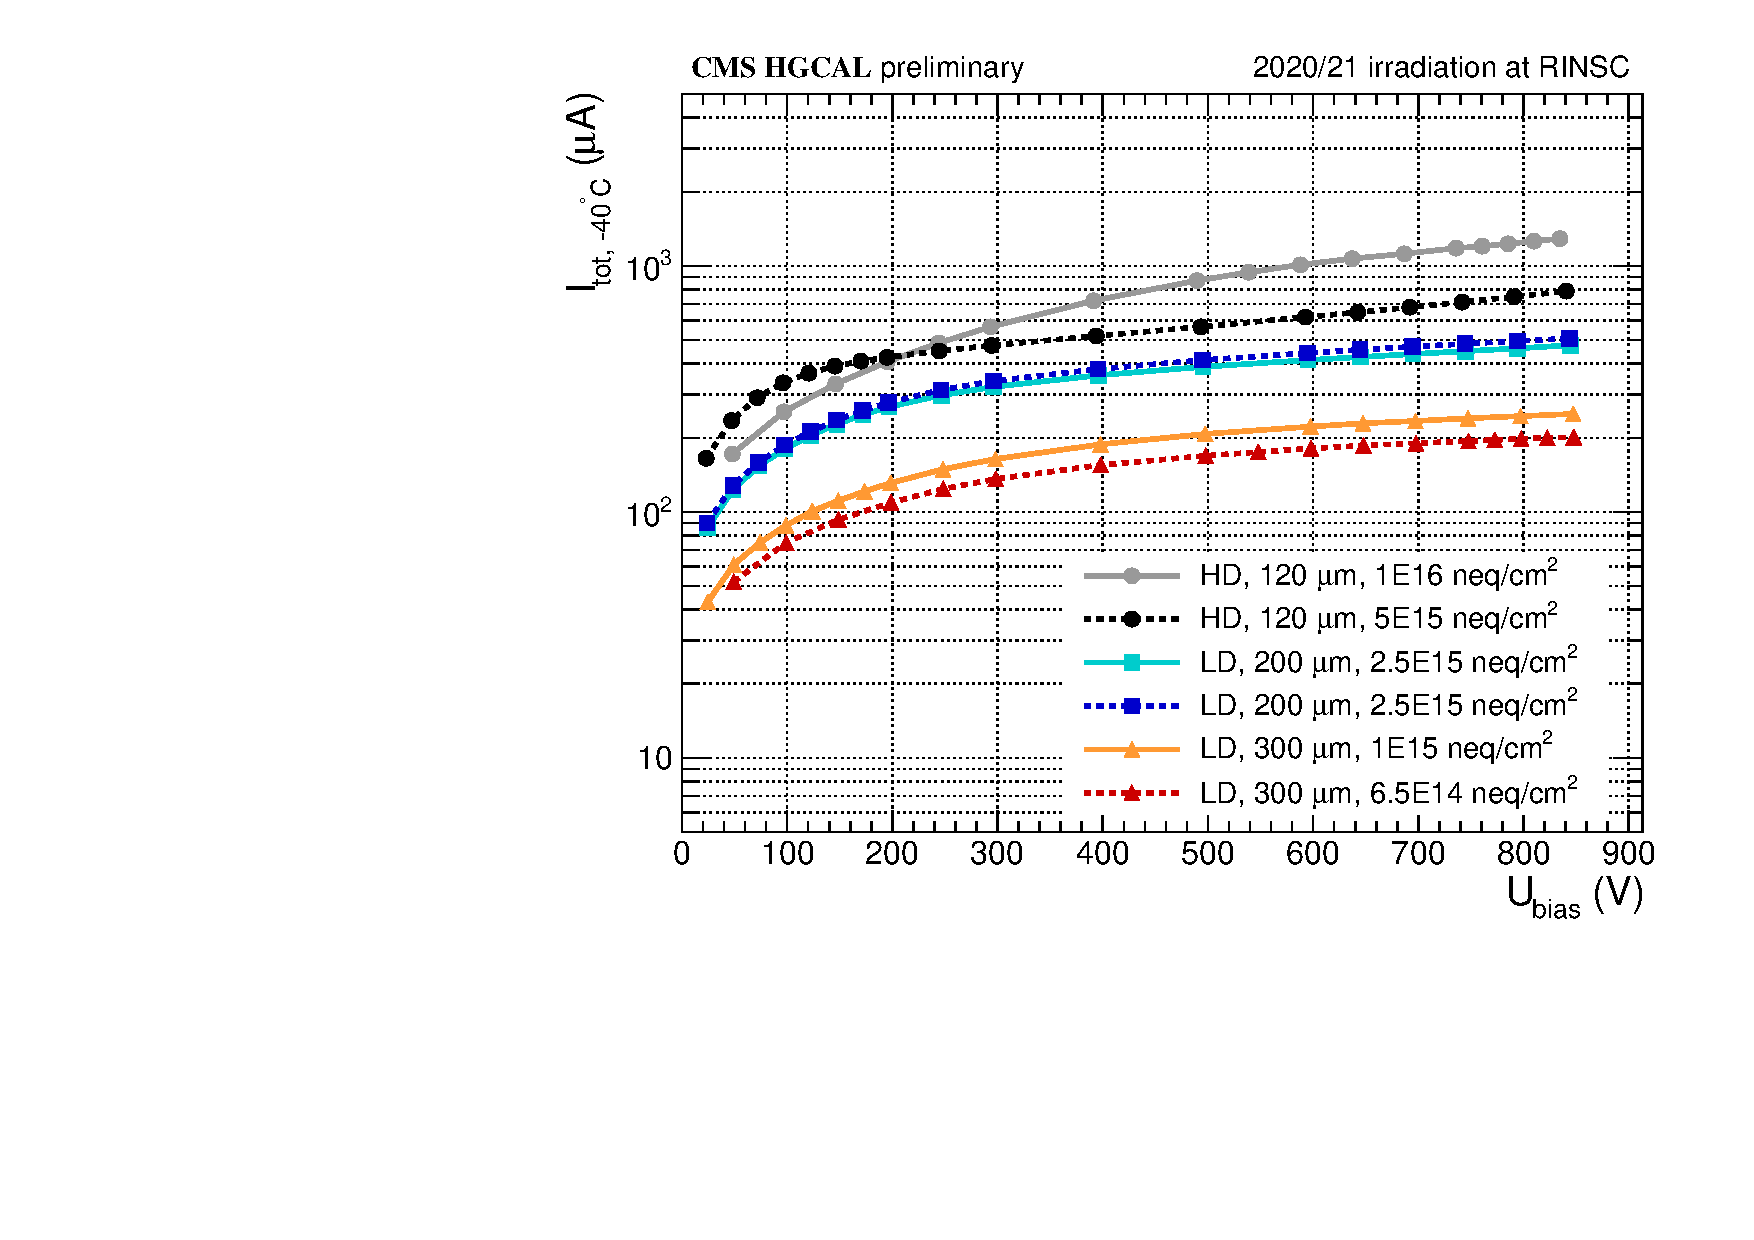
\includegraphics[width=0.999\textwidth]{plots/total_iv/total_current_IV.pdf}
		\subcaption{
		}
		\label{plot:tot_IV_good}
	\end{subfigure}
	\hfill
	\begin{subfigure}[b]{0.49\textwidth}
		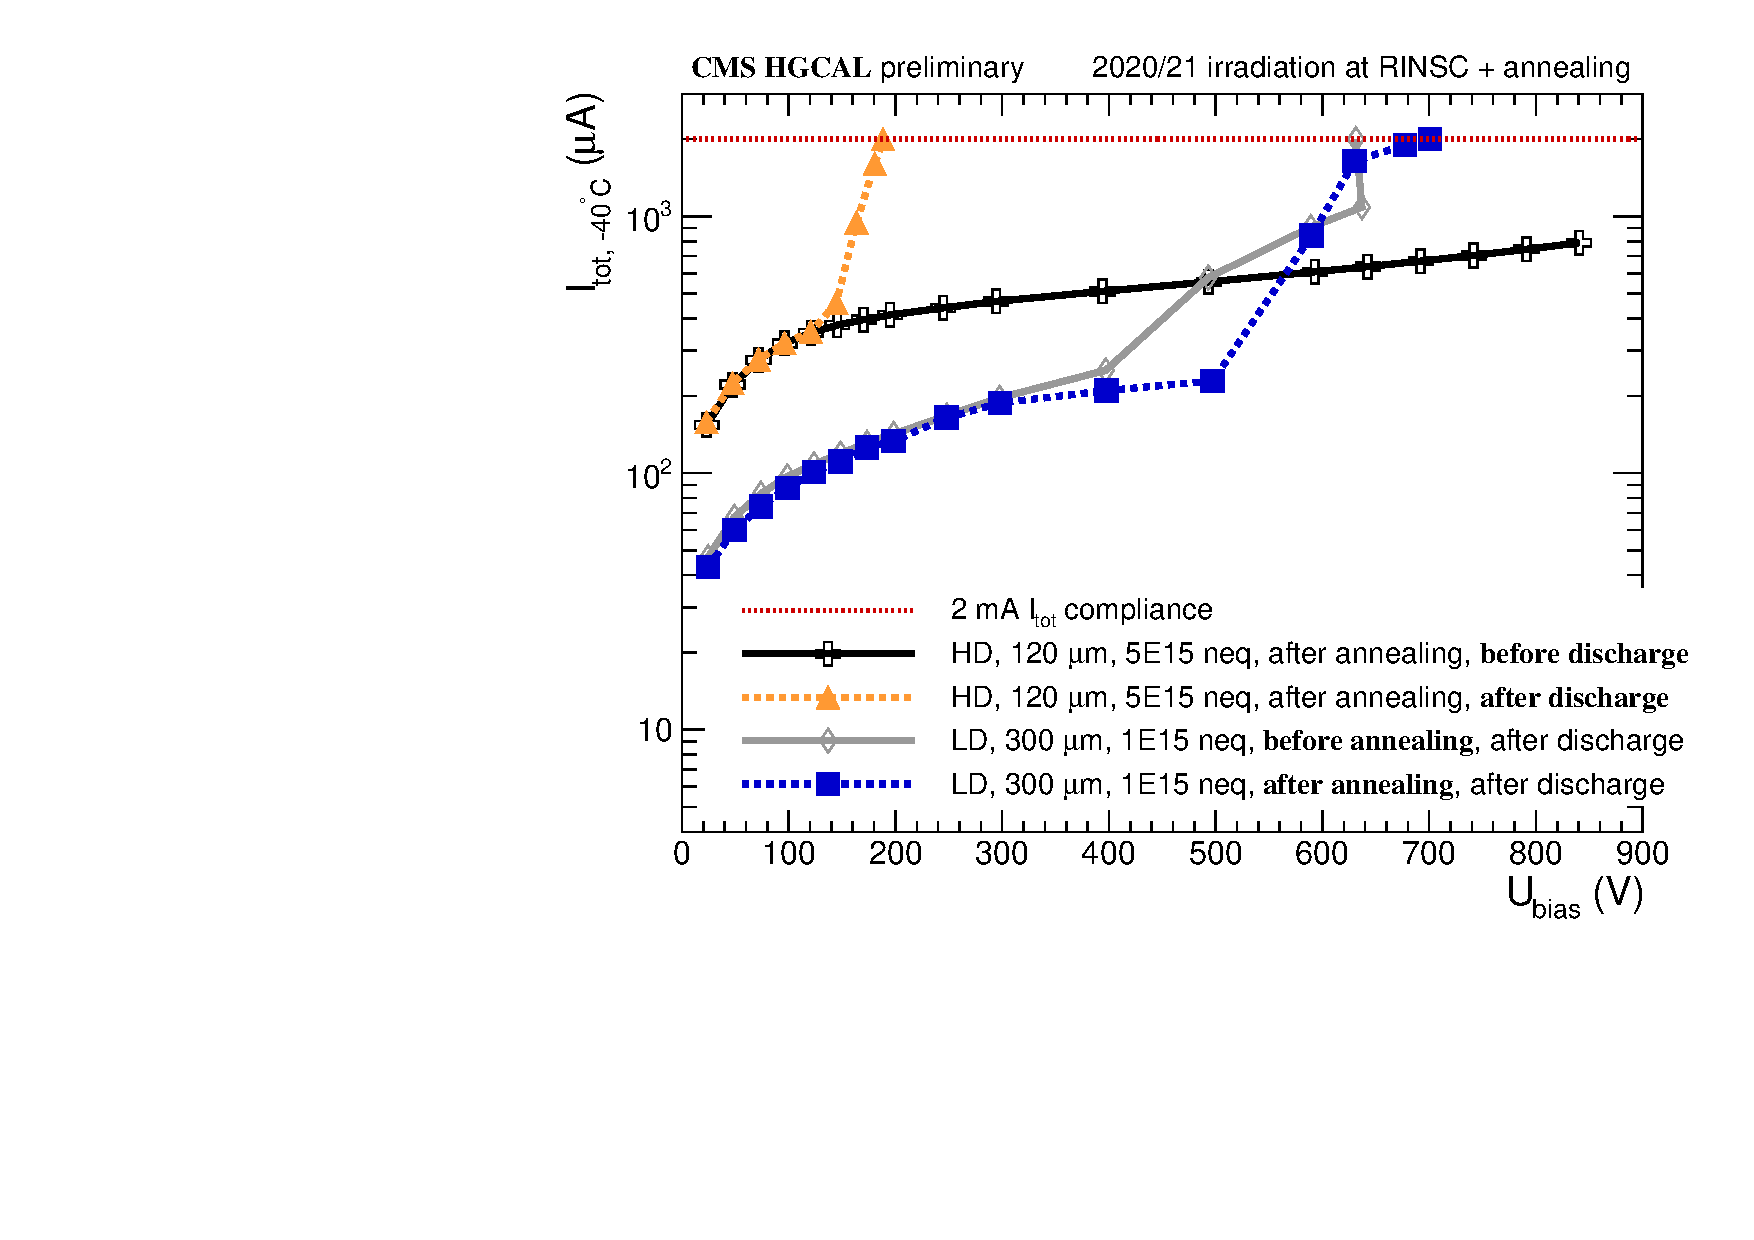
\includegraphics[width=0.999\textwidth]{plots/total_iv/total_current_IV_bad.pdf}
		\subcaption{
		}
		\label{plot:tot_IV_bad}
	\end{subfigure}
	\caption{
		Full-wafer leakage currents after additional annealing to \SI{80}{\min} at \SI{60}{\celsius}. Measurements were taken at \SI{-40}{\celsius} ($\text{I}_\text{tot, \SI{-40}{\celsius}}$) and for different effective bias voltages ($\text{U}_\text{bias}$). 
		Shown are (a) two representative "good" (passing the sensor quality criteria) sensors from two different irradiation rounds, and (b) two examples of "bad" (failing the sensor quality criteria), i.e. sensors with sudden leakage current increase.
	}
\end{figure}



\subsection{Per-Pad Leakage Currents}
\label{subsec:QA_Ipad}

\begin{itemize}
	\item Per-pad currents interpolated to \SI{600}{\volt} for representative good sensors shown in~\ref{plot:iv_hexplot_3003,plot:iv_hexplot_3009,plot:iv_hexplot_0541_04,plot:iv_hexplot_2004,plot:iv_hexplot_1013,plot:iv_hexplot_1002}
	\item Provide table of approximate leakage currents
	\item Per-pad leakage currents for most pads at \SI{-40}{\celsius} do not exceed \SI{5}{\micro\ampere} compliance
	\item Profile is visible, could be attributed to fluence profile
	\item Relative current increase from \SI{600}{\volt} to \SI{850}{\volt} does not exceed limitations, cf. for one full pad on different sensors, cf.~\ref{plot:pad_IV_sensor}
	\item Current normalised by area constant, cf.~\ref{plot:pad_IV_sensor}
\end{itemize}

\begin{figure}
	\captionsetup[subfigure]{aboveskip=-1pt,belowskip=-1pt}
	\centering
	\begin{subfigure}[b]{0.32\textwidth}
		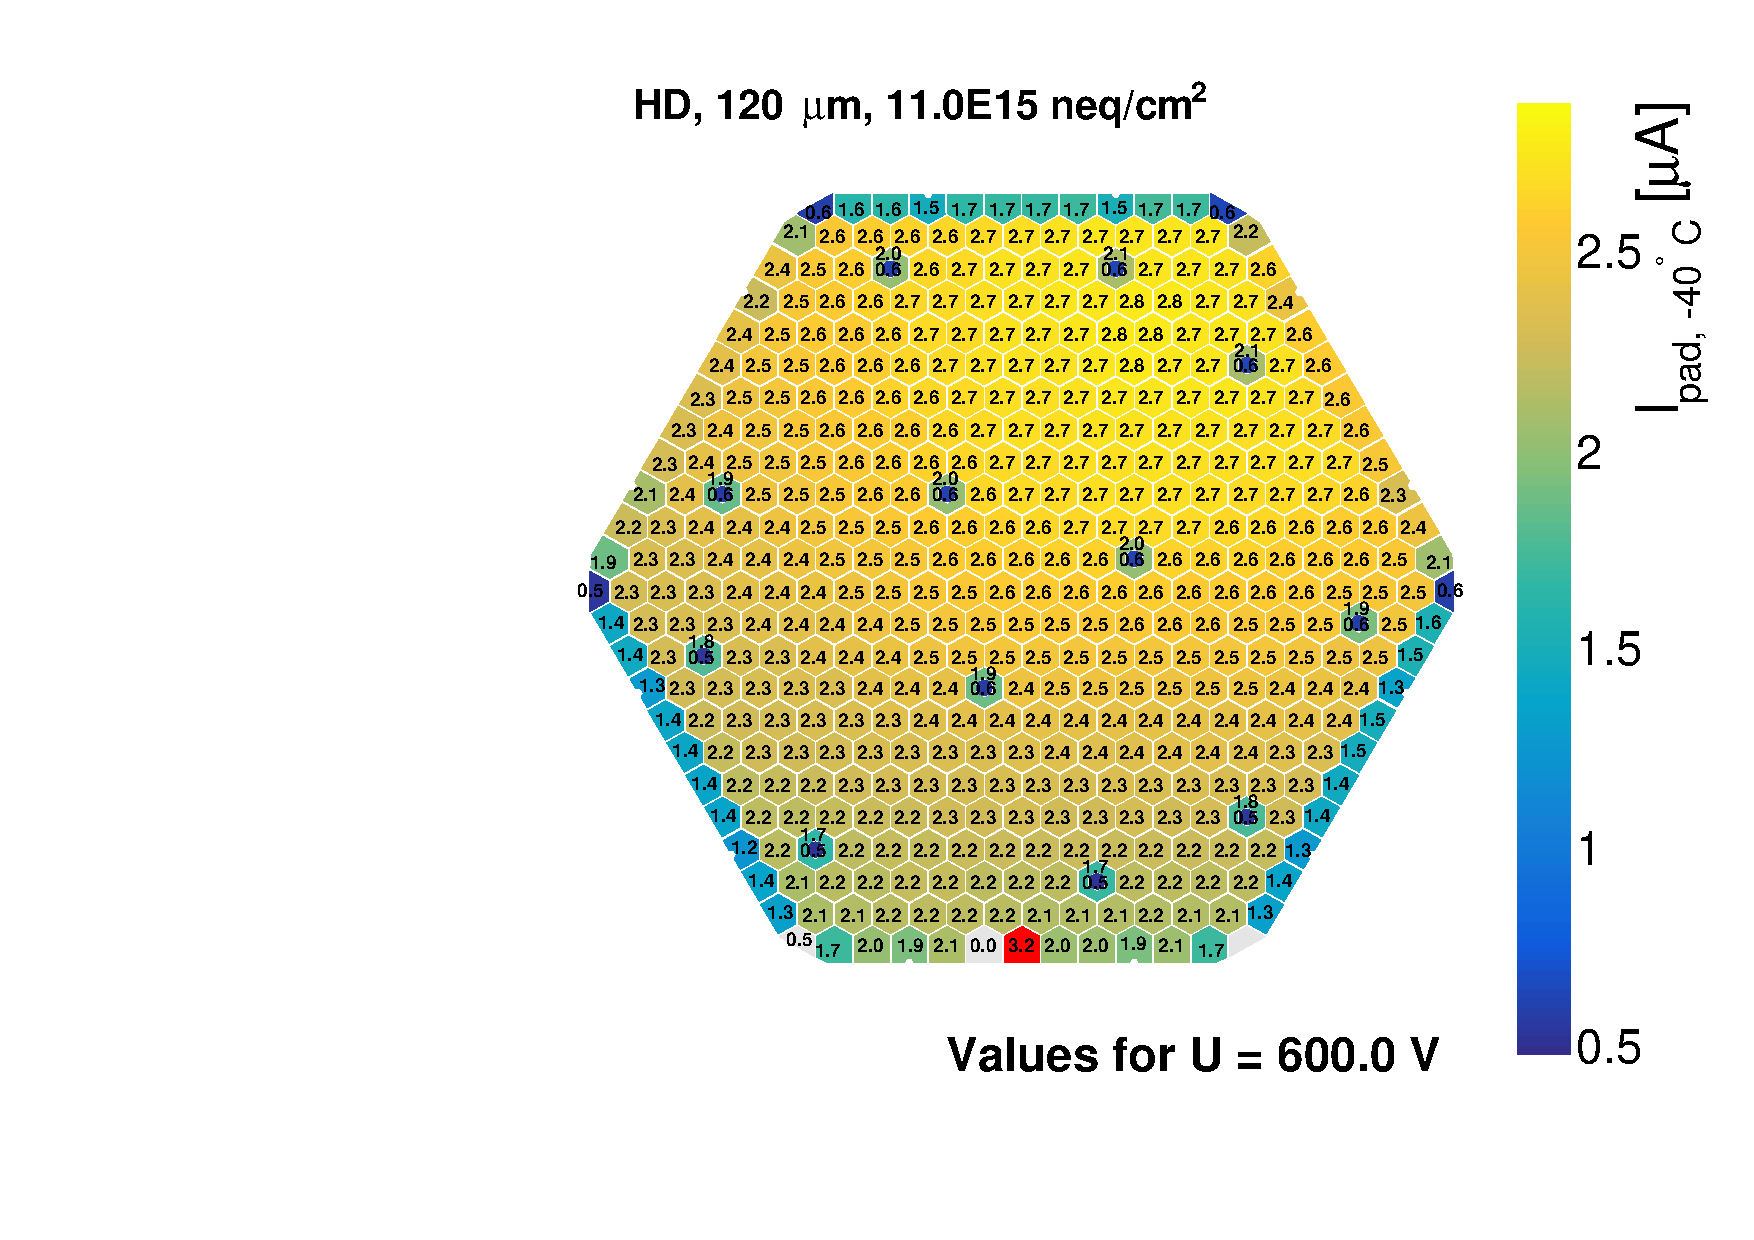
\includegraphics[width=0.999\textwidth]{plots/iv_hexplots/3003.pdf}
		\subcaption{
		}
		\label{plot:iv_hexplot_3003}
	\end{subfigure}
	\hfill
	\begin{subfigure}[b]{0.32\textwidth}
		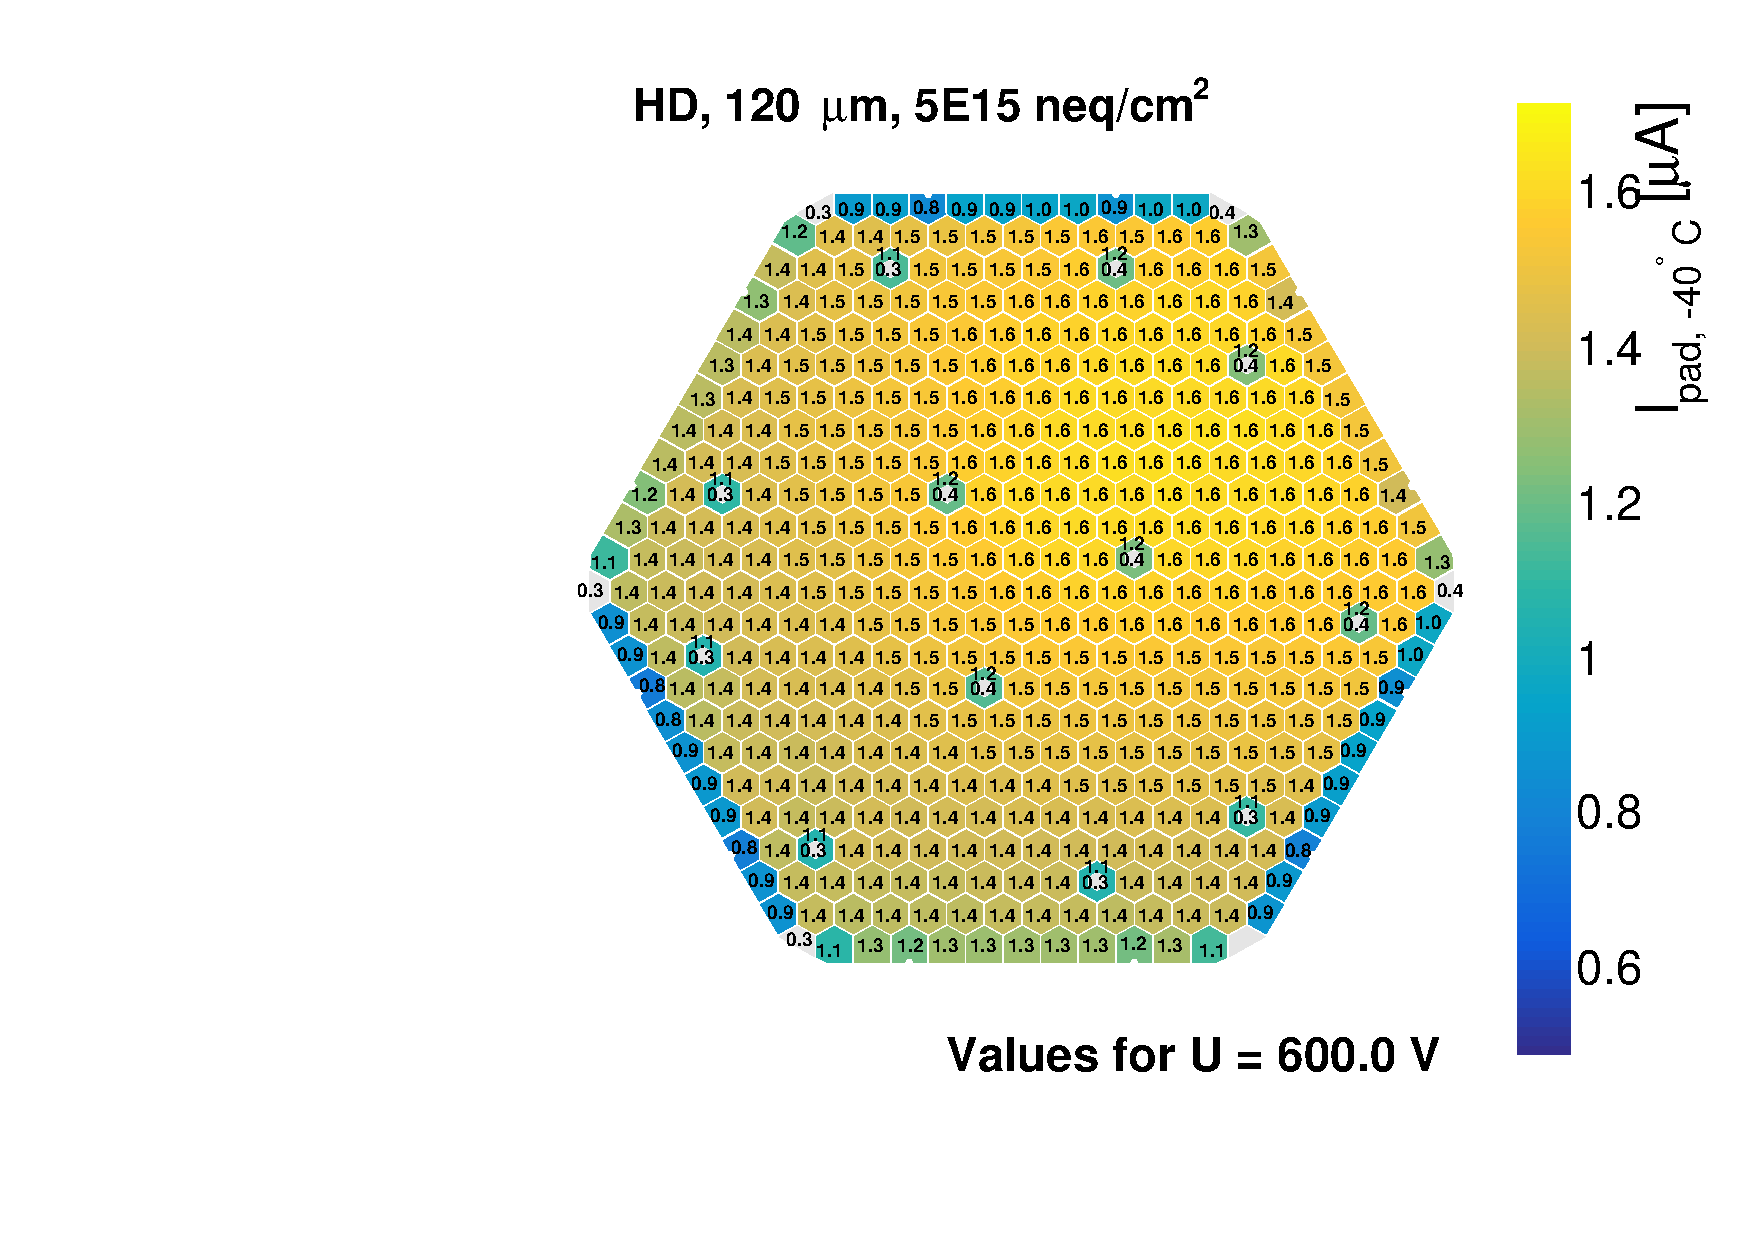
\includegraphics[width=0.999\textwidth]{plots/iv_hexplots/3009.pdf}
		\subcaption{
		}
		\label{plot:iv_hexplot_3009}
	\end{subfigure}
	\hfill
	\begin{subfigure}[b]{0.32\textwidth}
		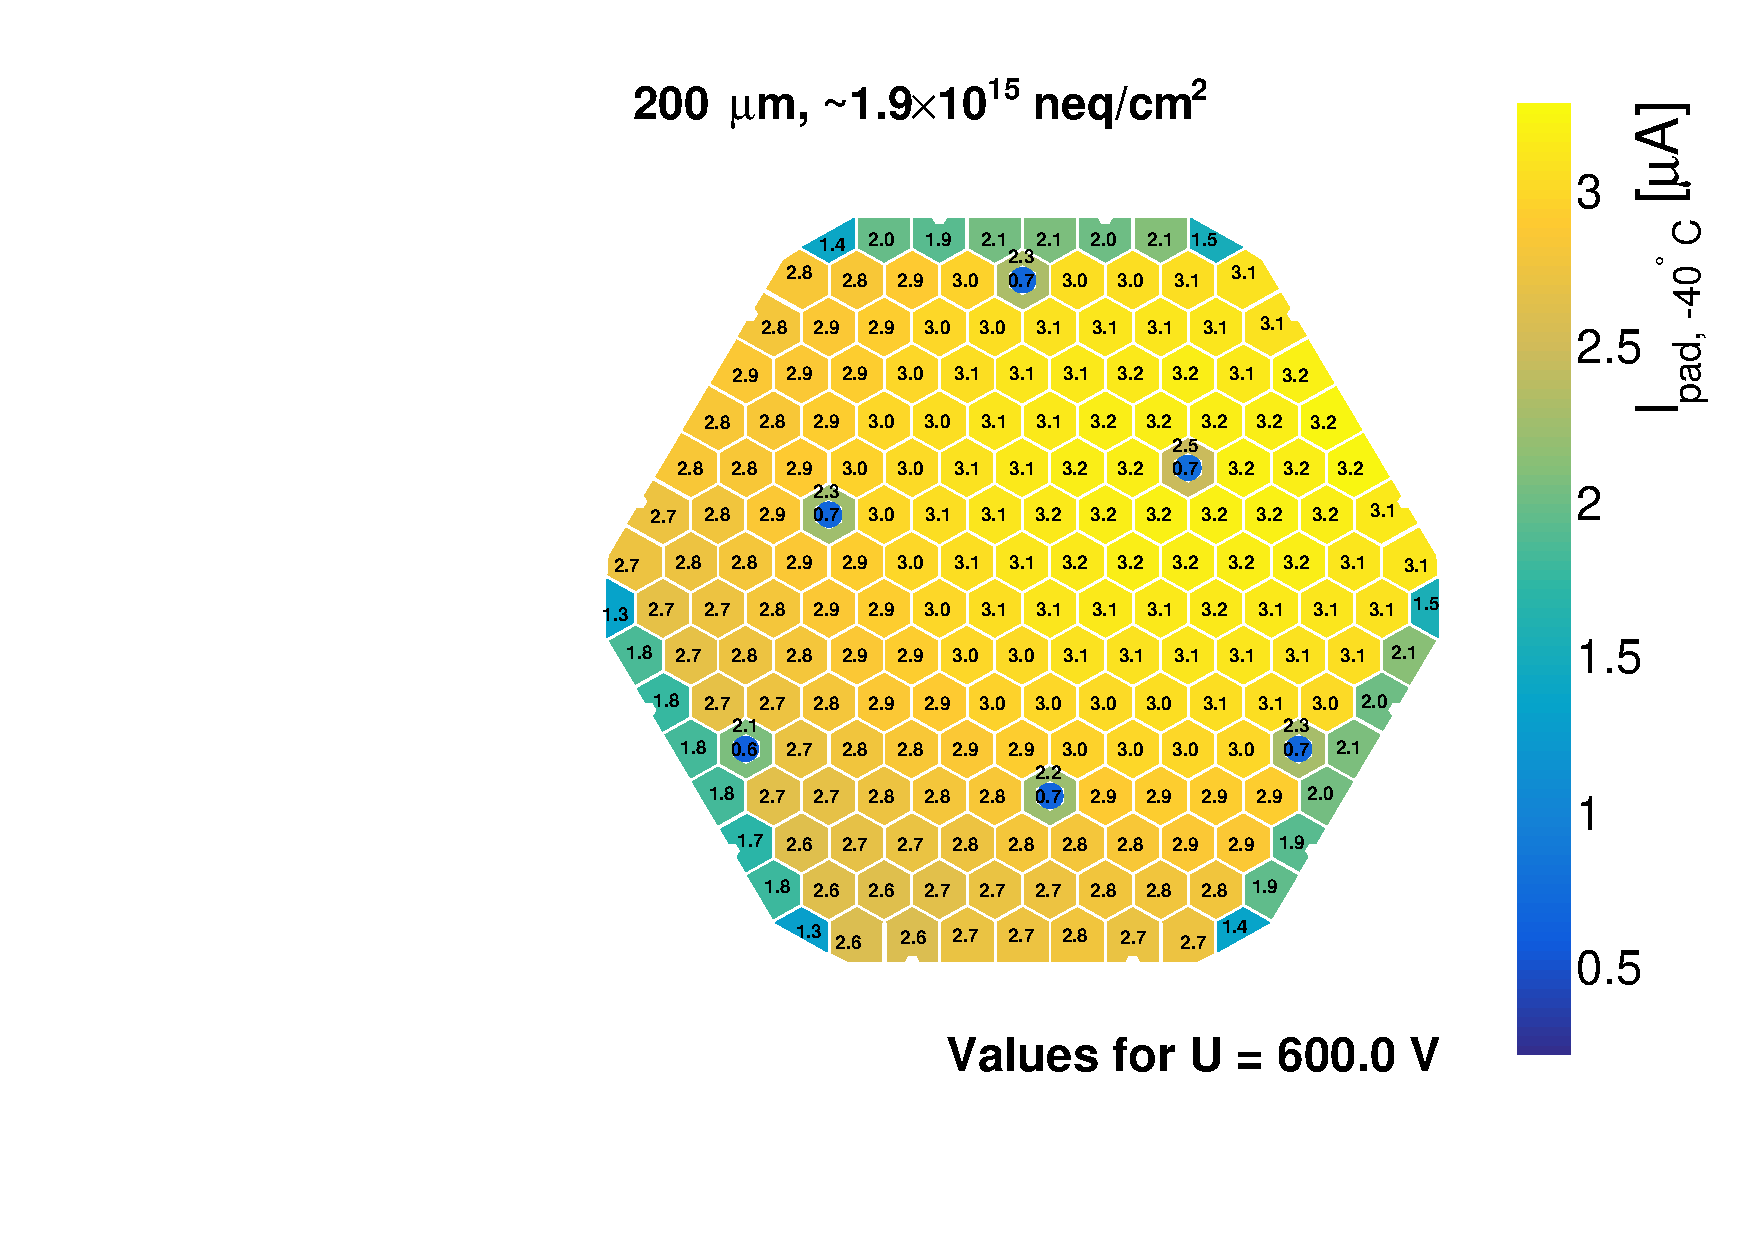
\includegraphics[width=0.999\textwidth]{plots/iv_hexplots/0541_04.pdf}
		\subcaption{
		}
		\label{plot:iv_hexplot_0541_04}
	\end{subfigure}
	\hfill	
	\begin{subfigure}[b]{0.32\textwidth}
		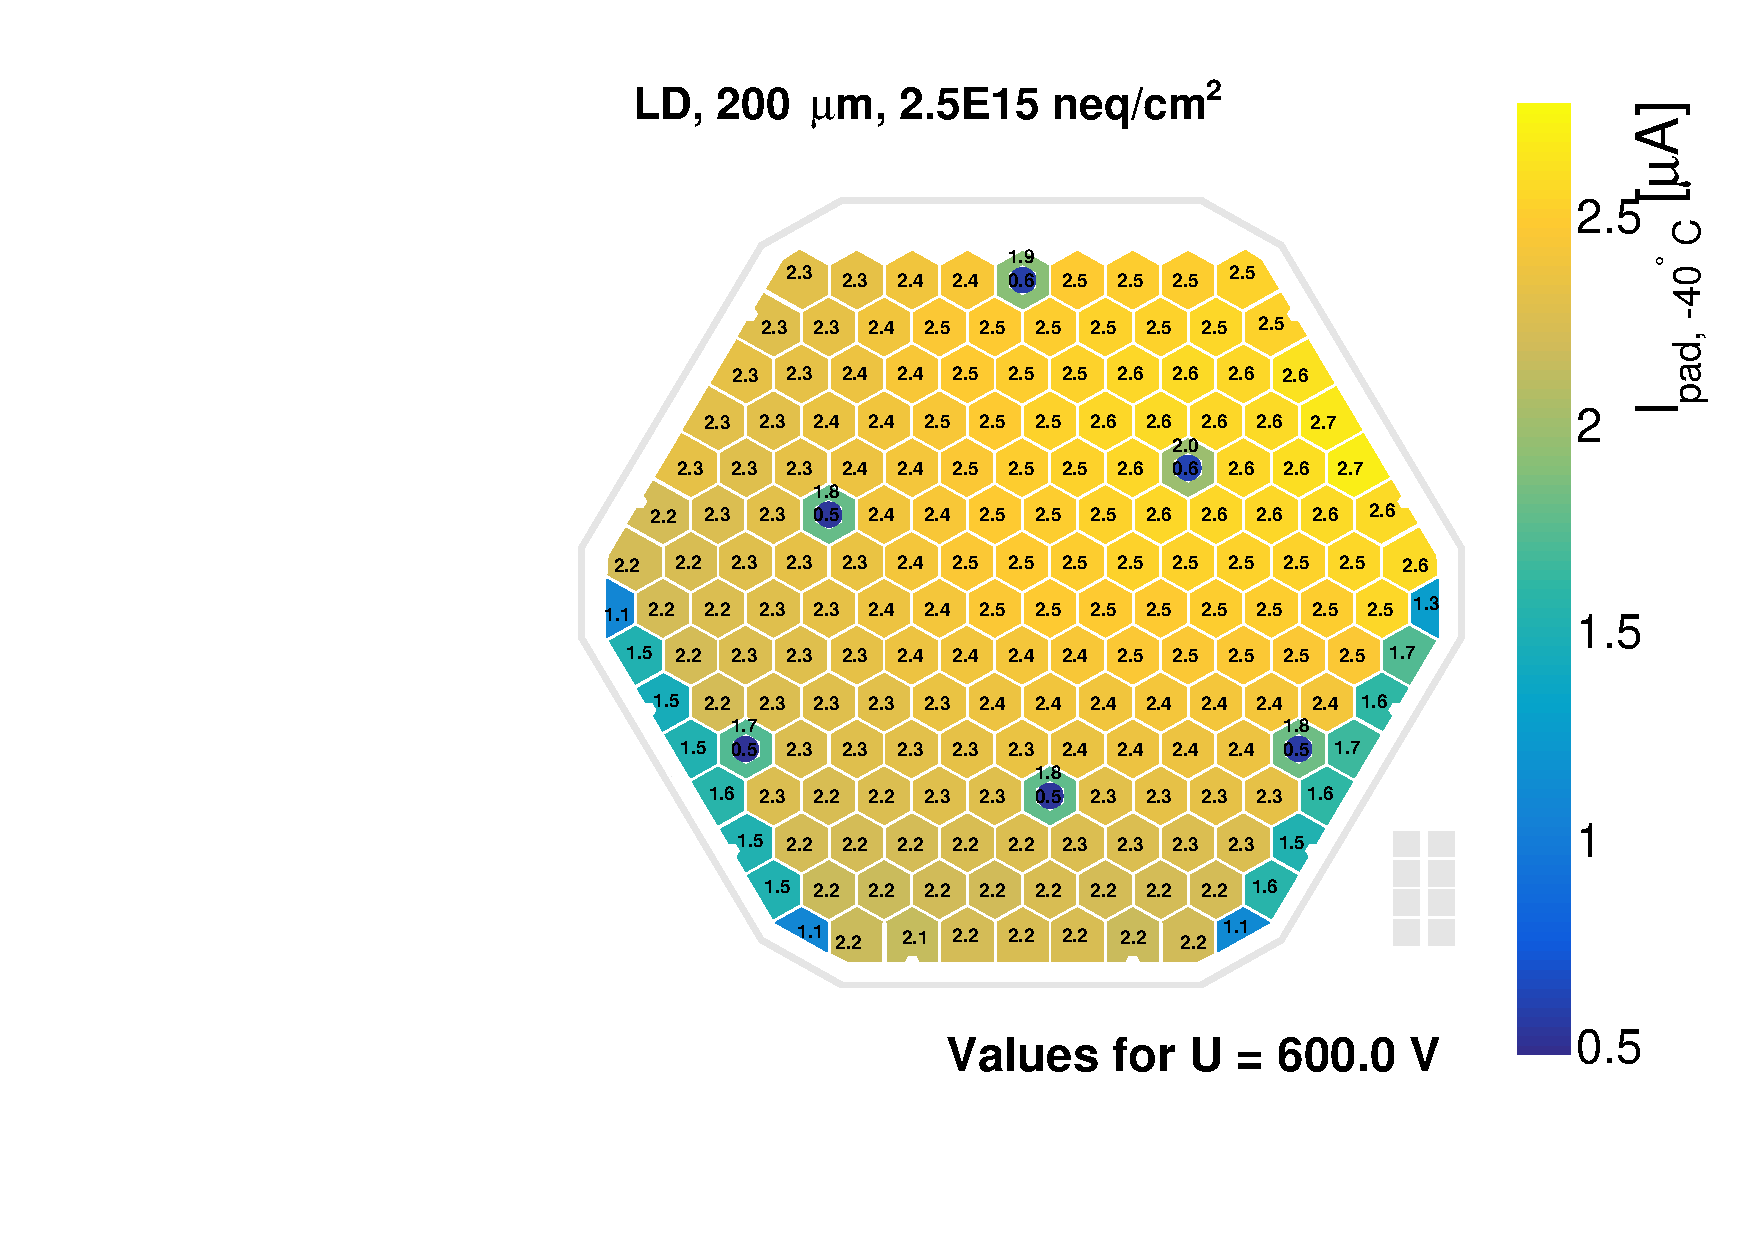
\includegraphics[width=0.999\textwidth]{plots/iv_hexplots/2004.pdf}
		\subcaption{
		}
		\label{plot:iv_hexplot_2004}
	\end{subfigure}
	\hfill
	\begin{subfigure}[b]{0.32\textwidth}
		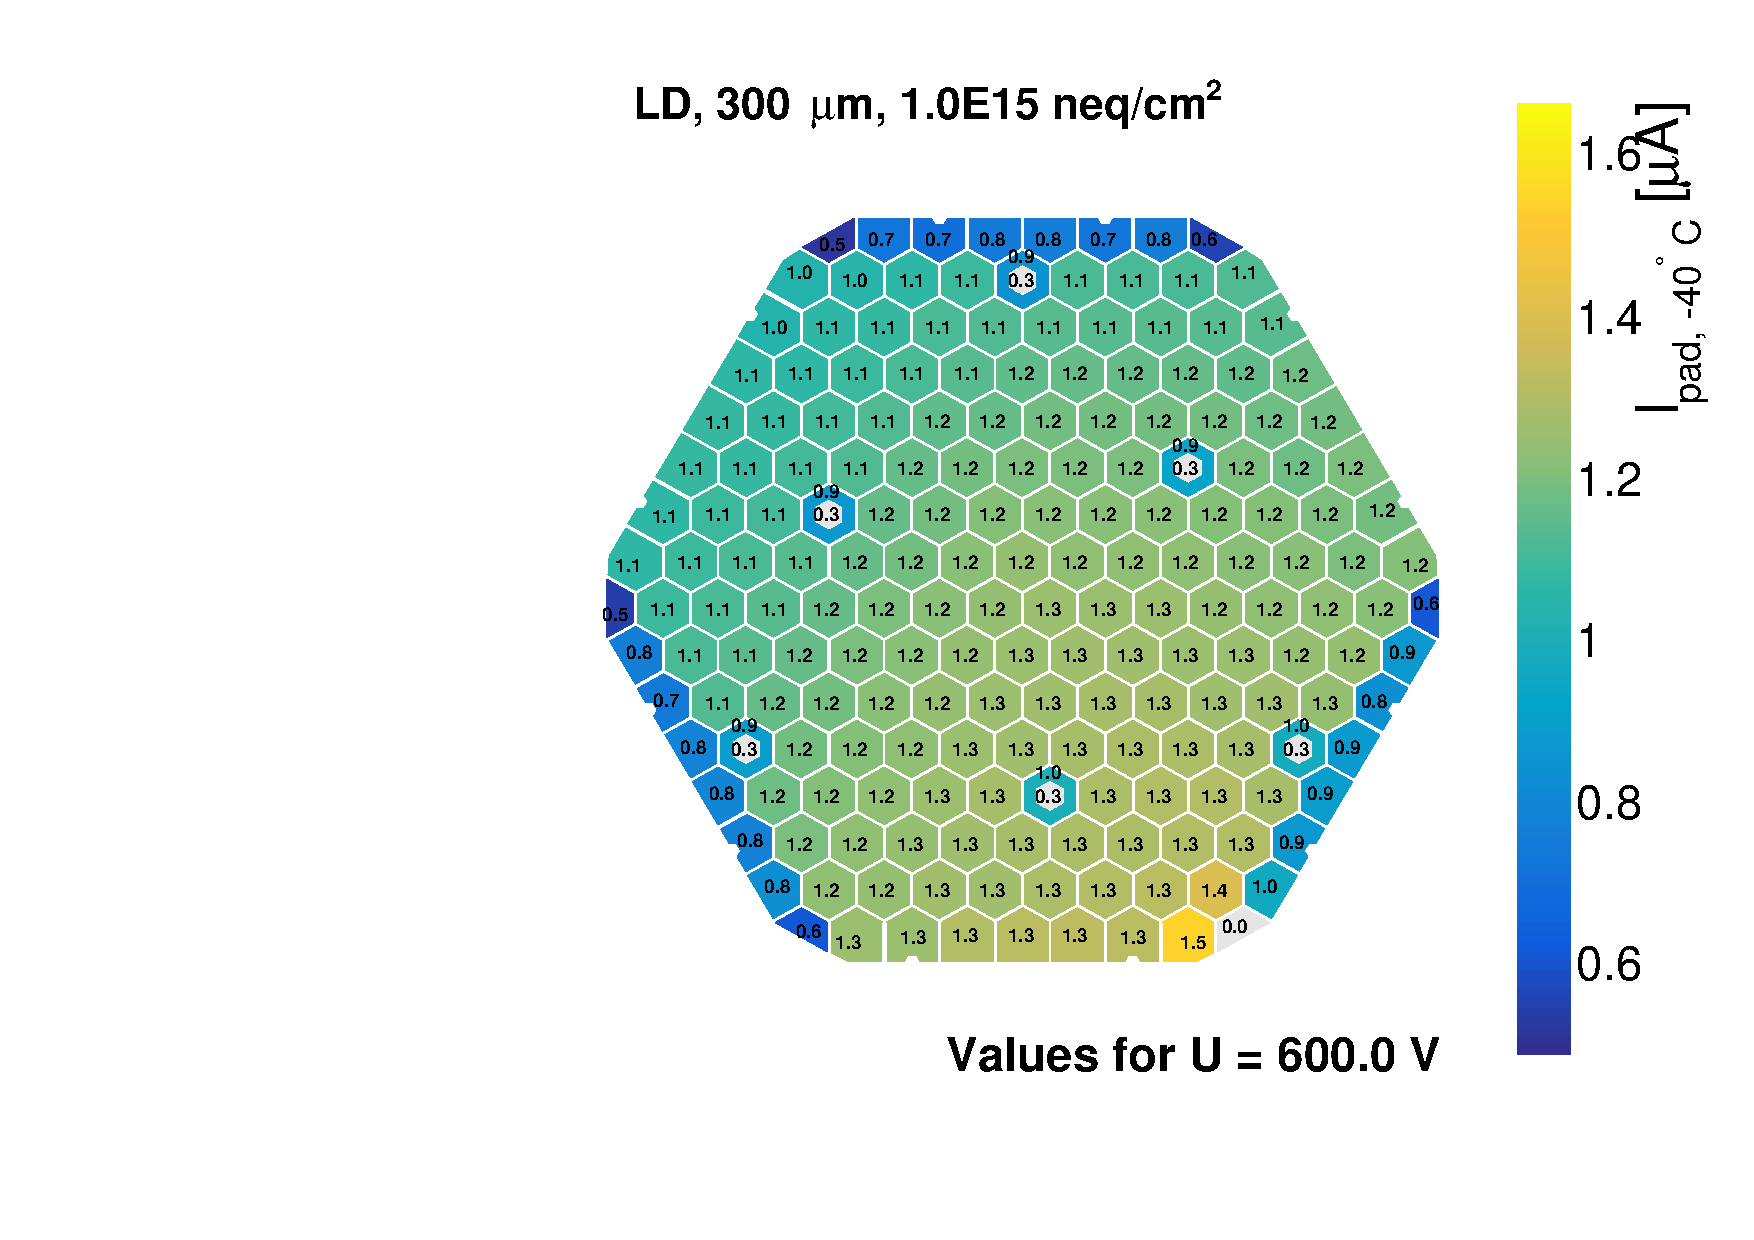
\includegraphics[width=0.999\textwidth]{plots/iv_hexplots/1013.pdf}
		\subcaption{
		}
		\label{plot:iv_hexplot_1013}
	\end{subfigure}
	\hfill
	\begin{subfigure}[b]{0.32\textwidth}
		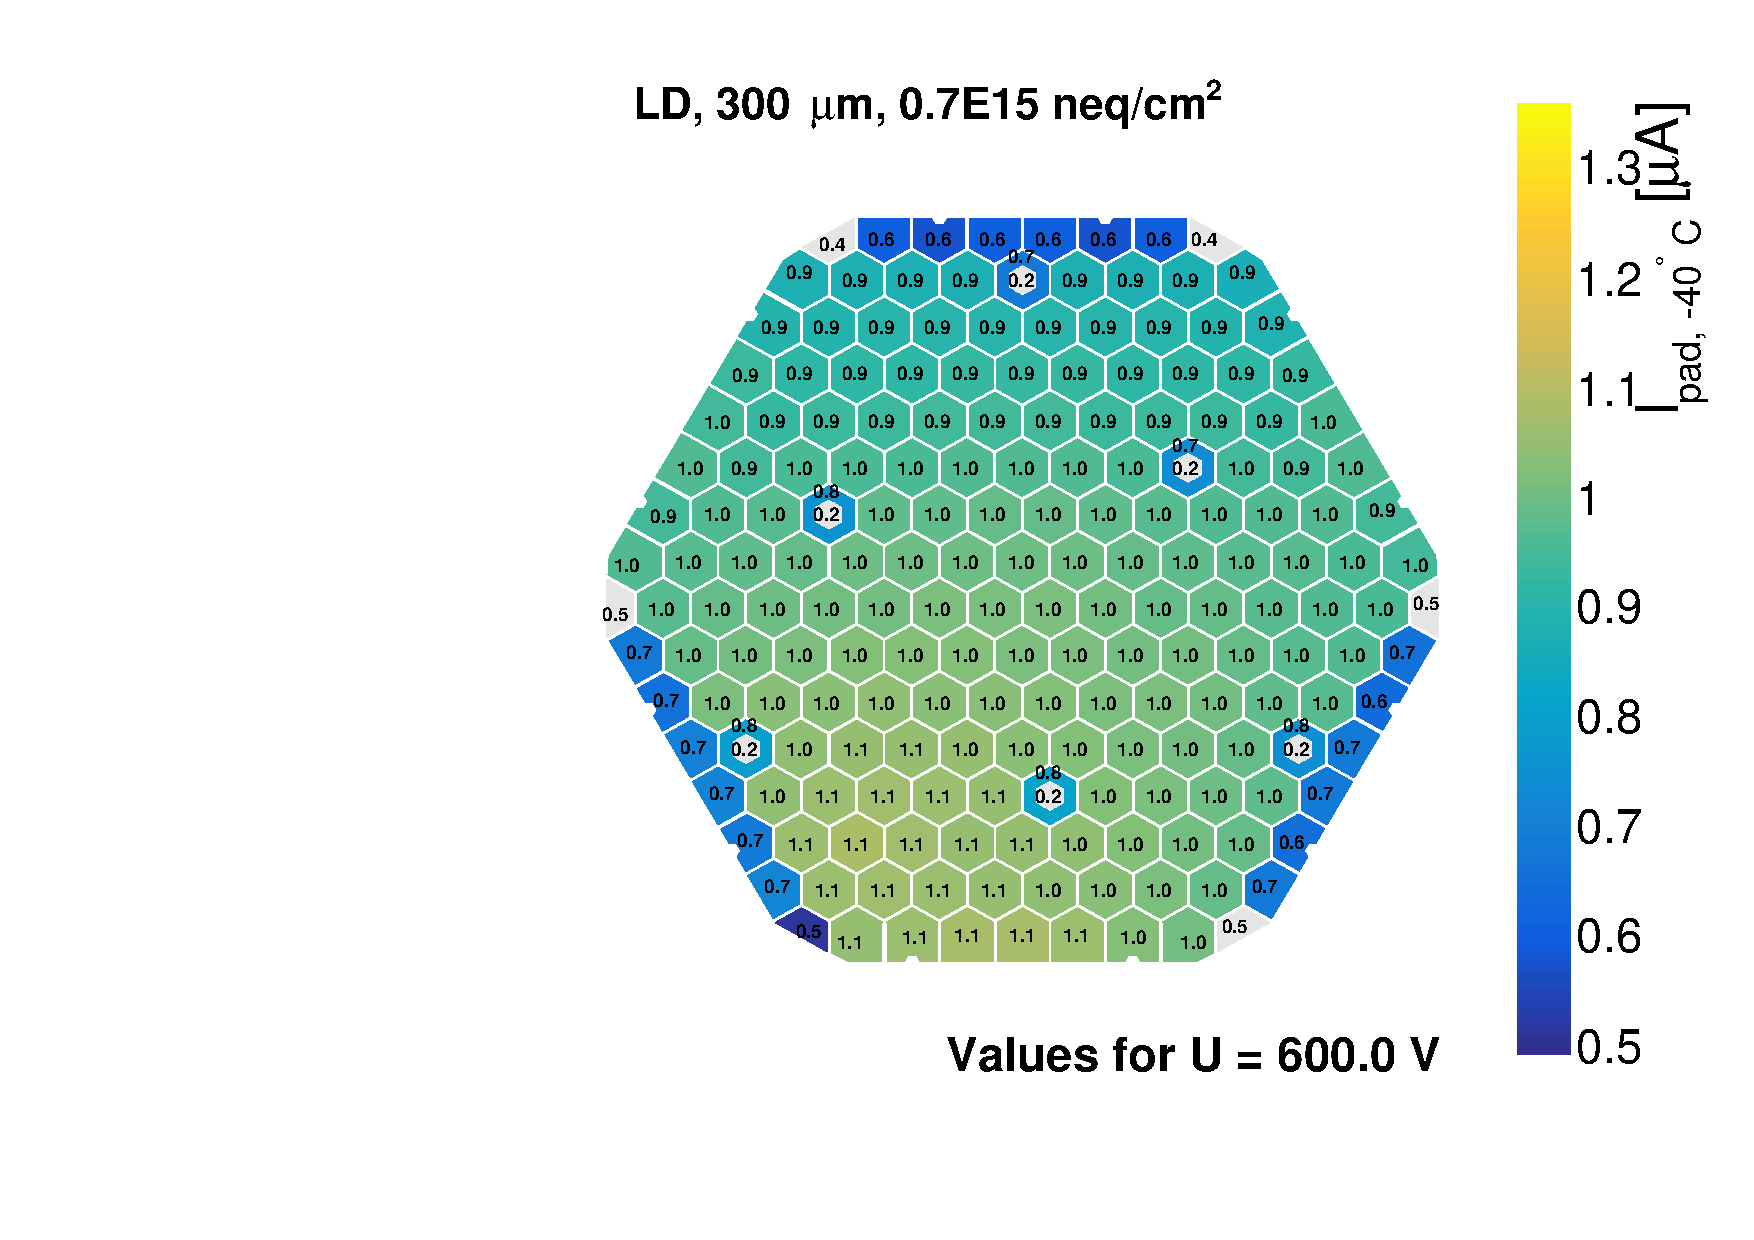
\includegraphics[width=0.999\textwidth]{plots/iv_hexplots/1002.pdf}
		\subcaption{
		}
		\label{plot:iv_hexplot_1002}
	\end{subfigure}	
	\label{plot:iv_hexplot}
	\caption{
		Per-pad leakage currents interpolated to an effective bias voltage of \SI{600}{\volt} for six representative sensors from all irradiation rounds.
		The chuck temperature profile is corrected for, cf.~\ref{appendix:chuck_temp}.
		Red- or white-colored edge pads correspond to well-understood (however undesired) measurement peculiarities, e.g. unconnected pogo pins.
		Note the different leakage current colour scales.
	}
\end{figure}


\begin{figure}
	\captionsetup[subfigure]{aboveskip=-1pt,belowskip=-1pt}
	\centering
	\begin{subfigure}[b]{0.49\textwidth}
		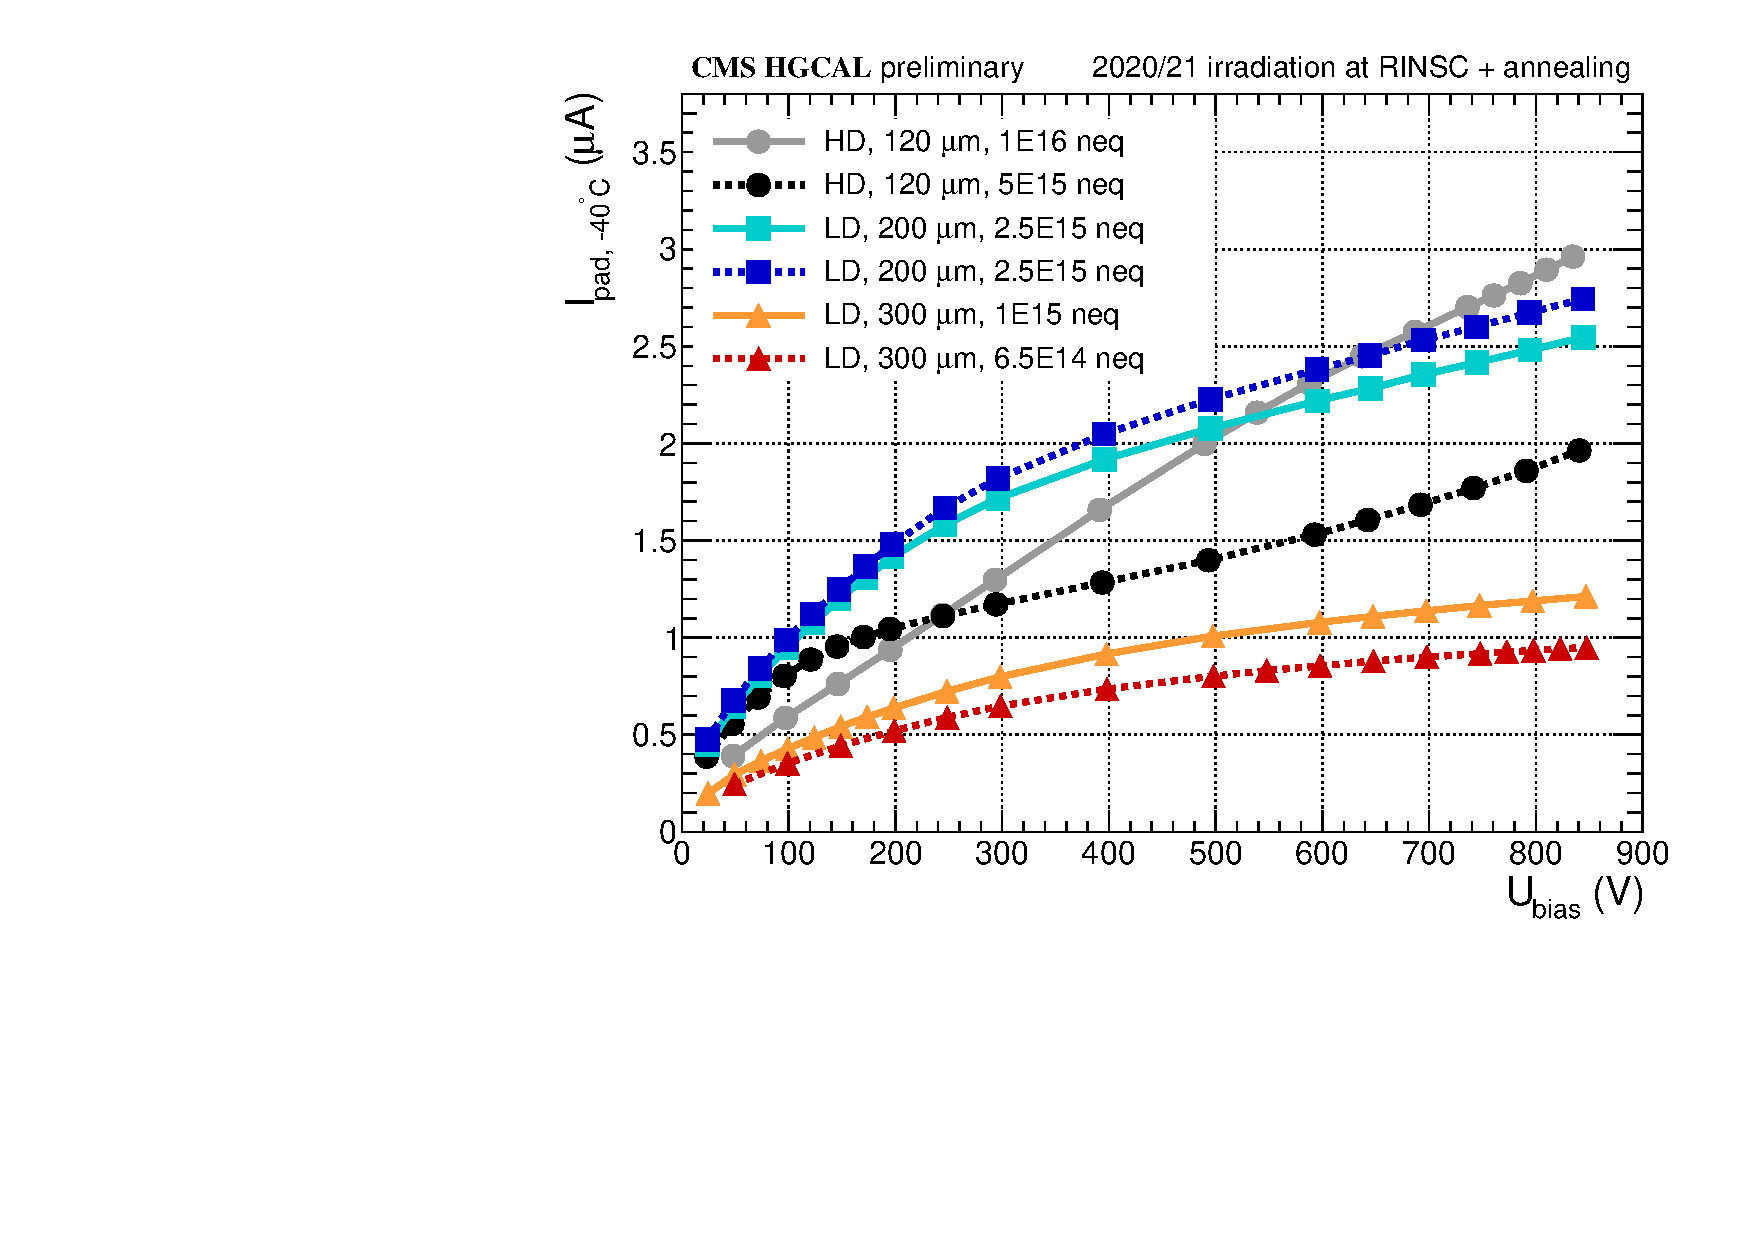
\includegraphics[width=0.999\textwidth]{plots/channel_iv/channel_IV_sensors_sensors.pdf}
		\subcaption{
		}
		\label{plot:pad_IV_sensor}
	\end{subfigure}
	\hfill
	\begin{subfigure}[b]{0.49\textwidth}
		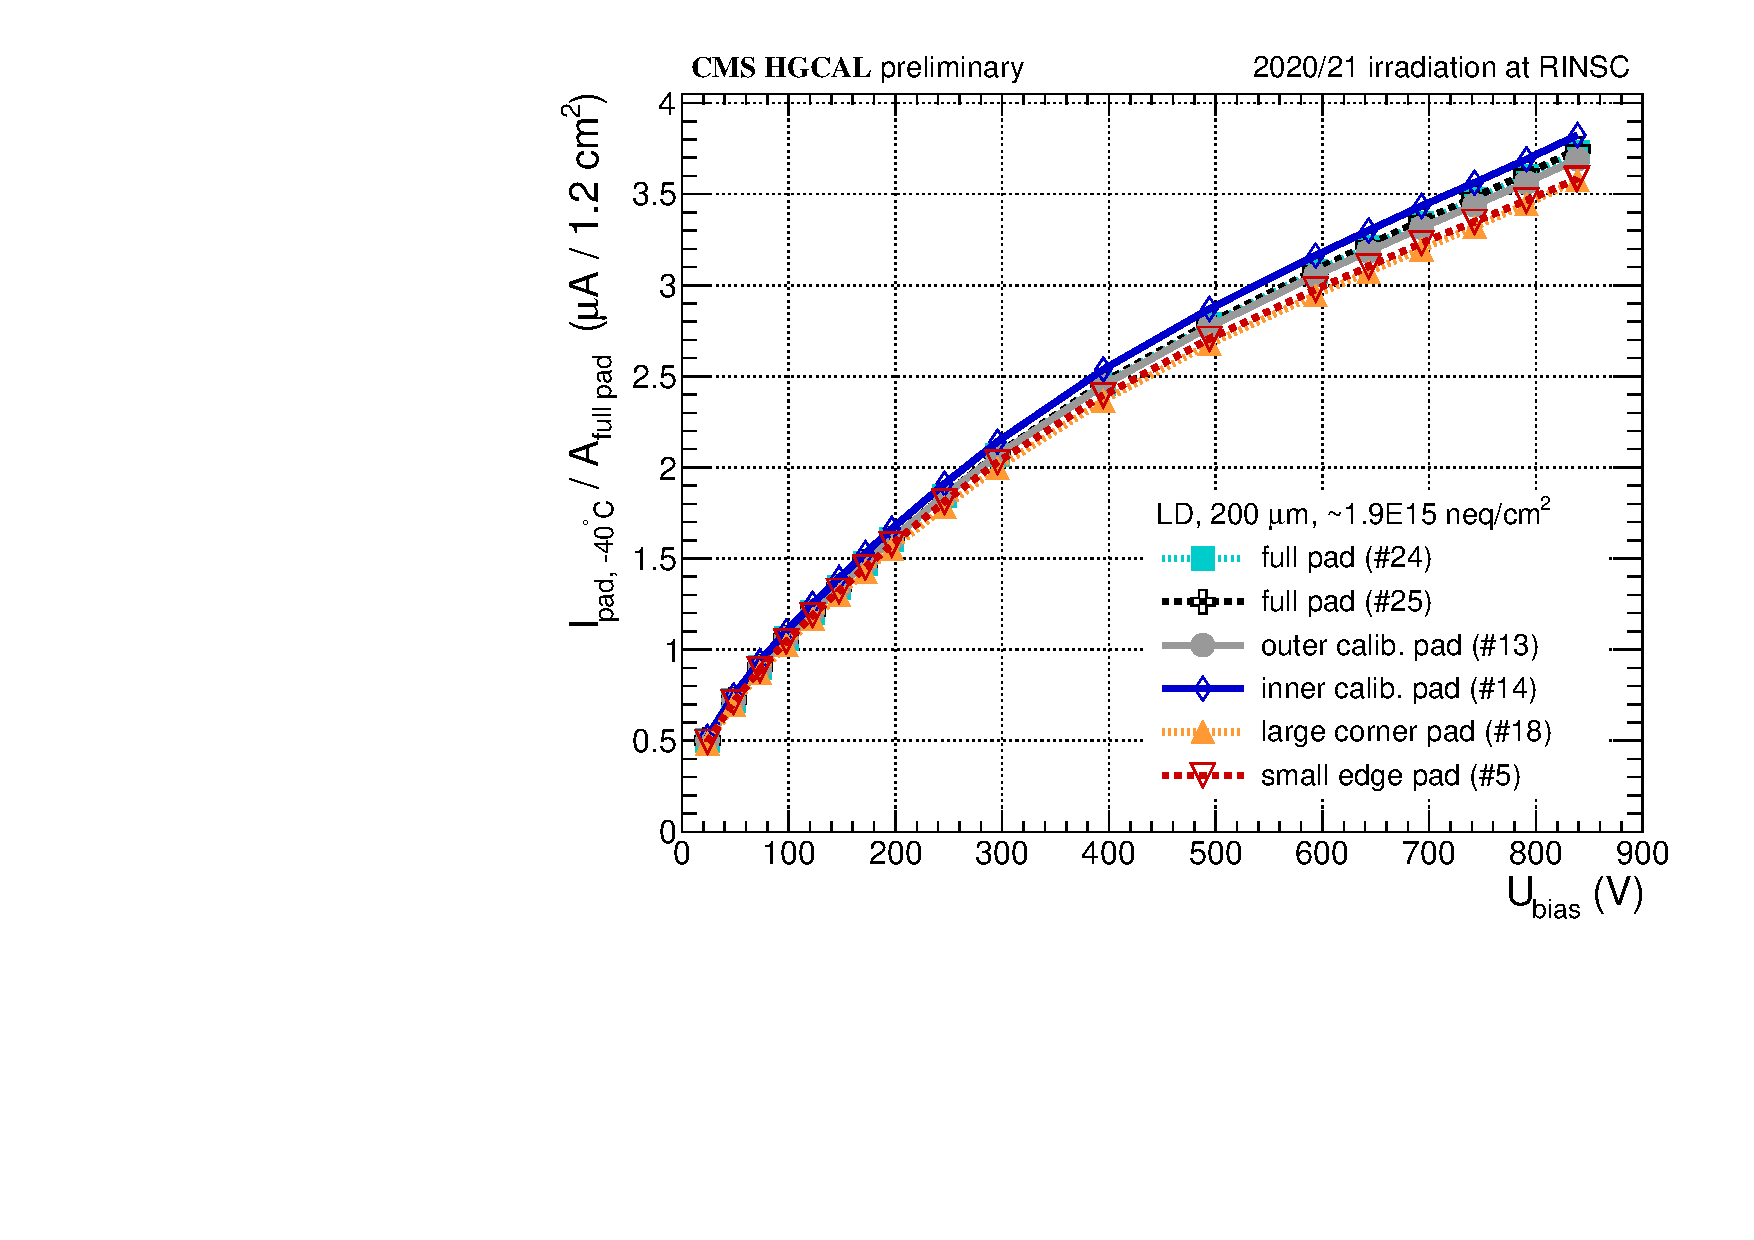
\includegraphics[width=0.999\textwidth]{plots/channel_iv/channel_IV_sensors_channels.pdf}
		\subcaption{
		}
		\label{plot:pad_IV_channels}
	\end{subfigure}
	\caption{
		Leakage currents as a function of the effective bias voltage (a) of one central pad on six good sensors from all irradiation rounds normalised to the respective currents at $U_\text{bias}=\SI{600}{\volt}$, 
		and (b) for different pads with different geometries on one example low density sensor normalised to the area of full hexagonal pads.
	}
\end{figure}



\subsection{Per-Pad Capacitance and Depletion Voltage}
\label{subsec:QA_Vdep}

\begin{itemize}
	\item Capacitances are open-corrected, serial definition, LCR frequency = 2kHz (reminder)
	\item Only slight dependence of capacitance on bias voltage in the tested regime, cf.~\ref{plot:pad_CV_sensor}
	\item Area- and thickness normalised end capacitance different for different sensors. Not clear why, no systematic trend w.r.t. fluence or so
	\item Capacitance dominated by bulk, area-normalised capacitance on one sensor = stable within 5 percent, interpad contributions can explain differences?, cf.~\ref{plot:pad_CV_channels}
	\item Depletion voltage, i.e. where final capacitance is reached, clearly differs between fluence scenarios and thicknesses, cf.~\ref{plot:pad_invCV_sensor}, provide table?
	\item Depletion voltage rather independent on pad geometry, cf.~\ref{plot:pad_invCV_channels}
	\item Depletion voltage hexplot shows profile, matches leakage current profile, quantified in~\ref{subsec:irradiation_Vdep}
\end{itemize}

\begin{figure}
	\captionsetup[subfigure]{aboveskip=-1pt,belowskip=-1pt}
	\centering
	\begin{subfigure}[b]{0.49\textwidth}
		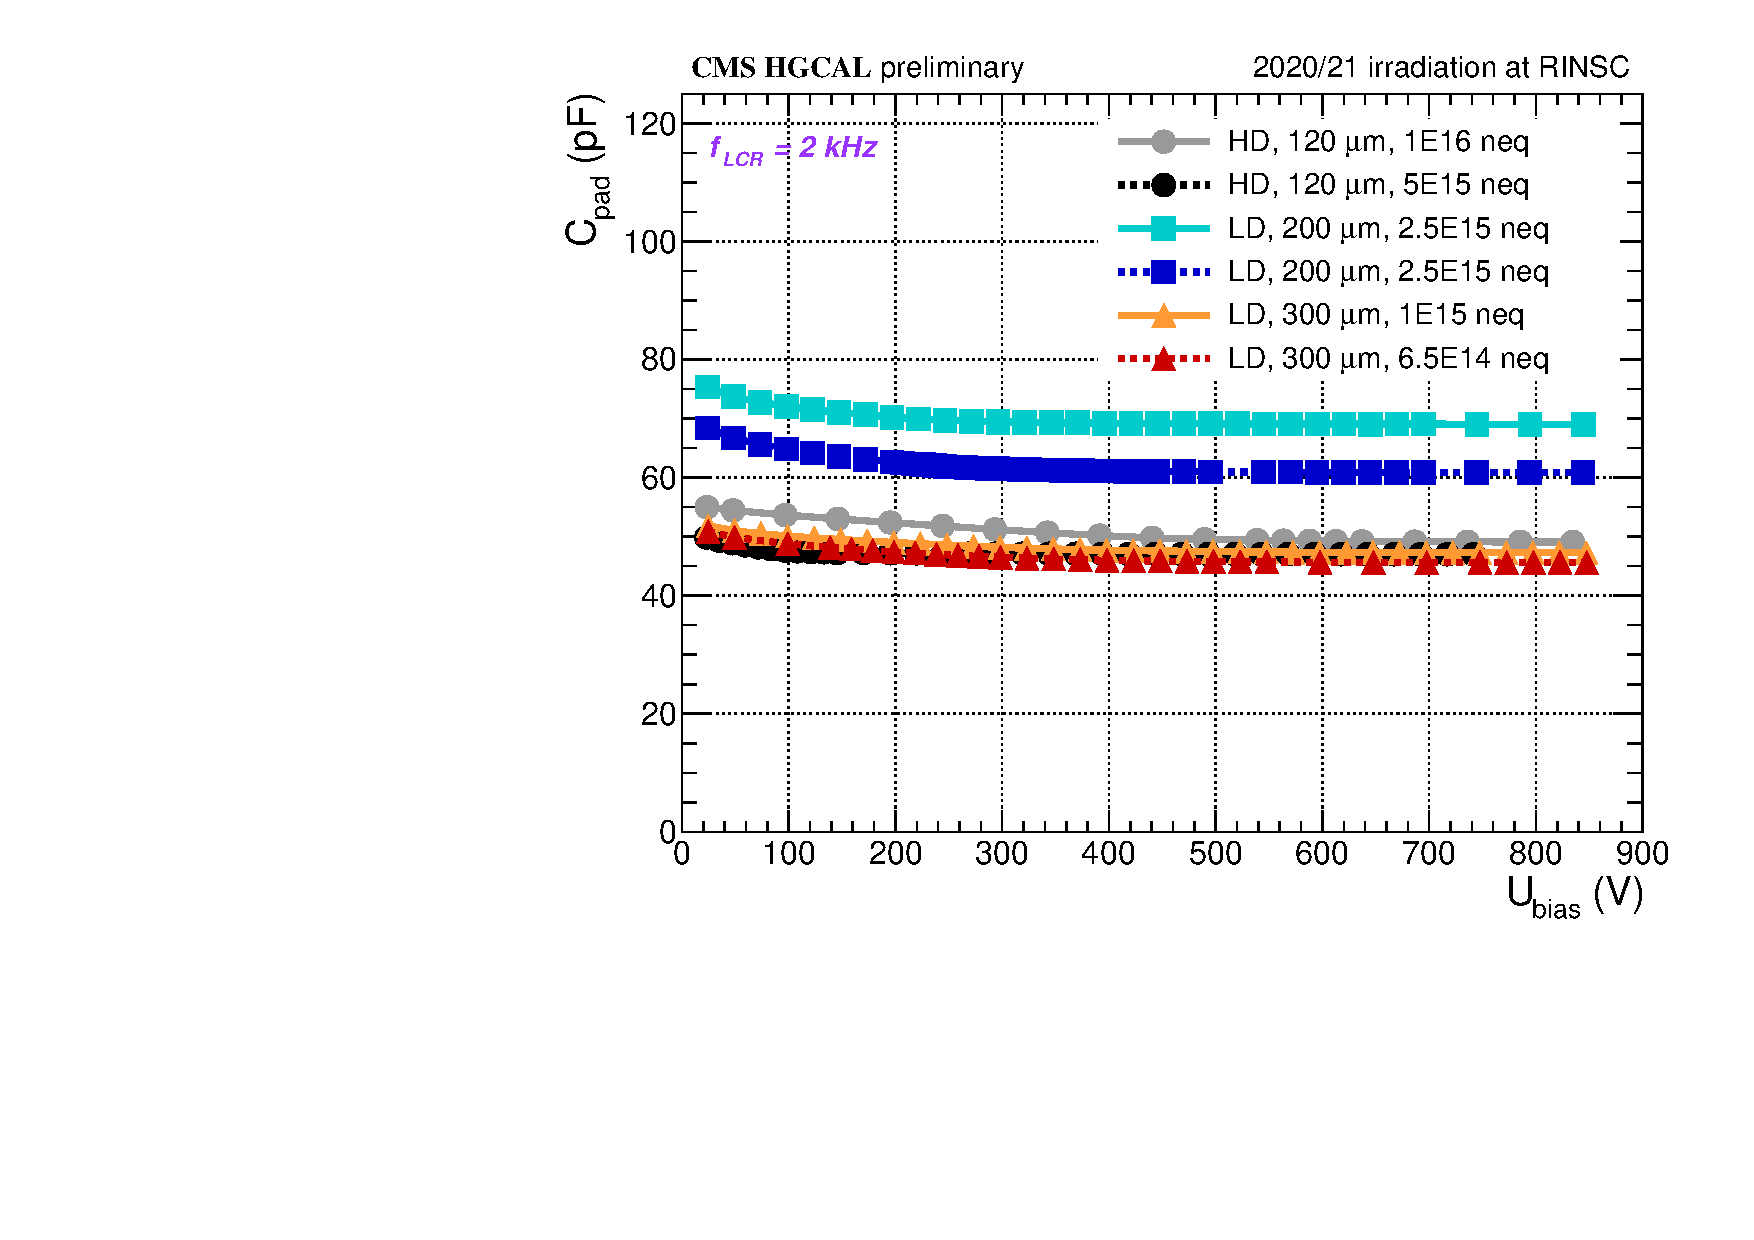
\includegraphics[width=0.999\textwidth]{plots/channel_cv/channel_CV_sensors_sensors.pdf}
		\subcaption{
		}
		\label{plot:pad_CV_sensor}
	\end{subfigure}
	\hfill
	\begin{subfigure}[b]{0.49\textwidth}
		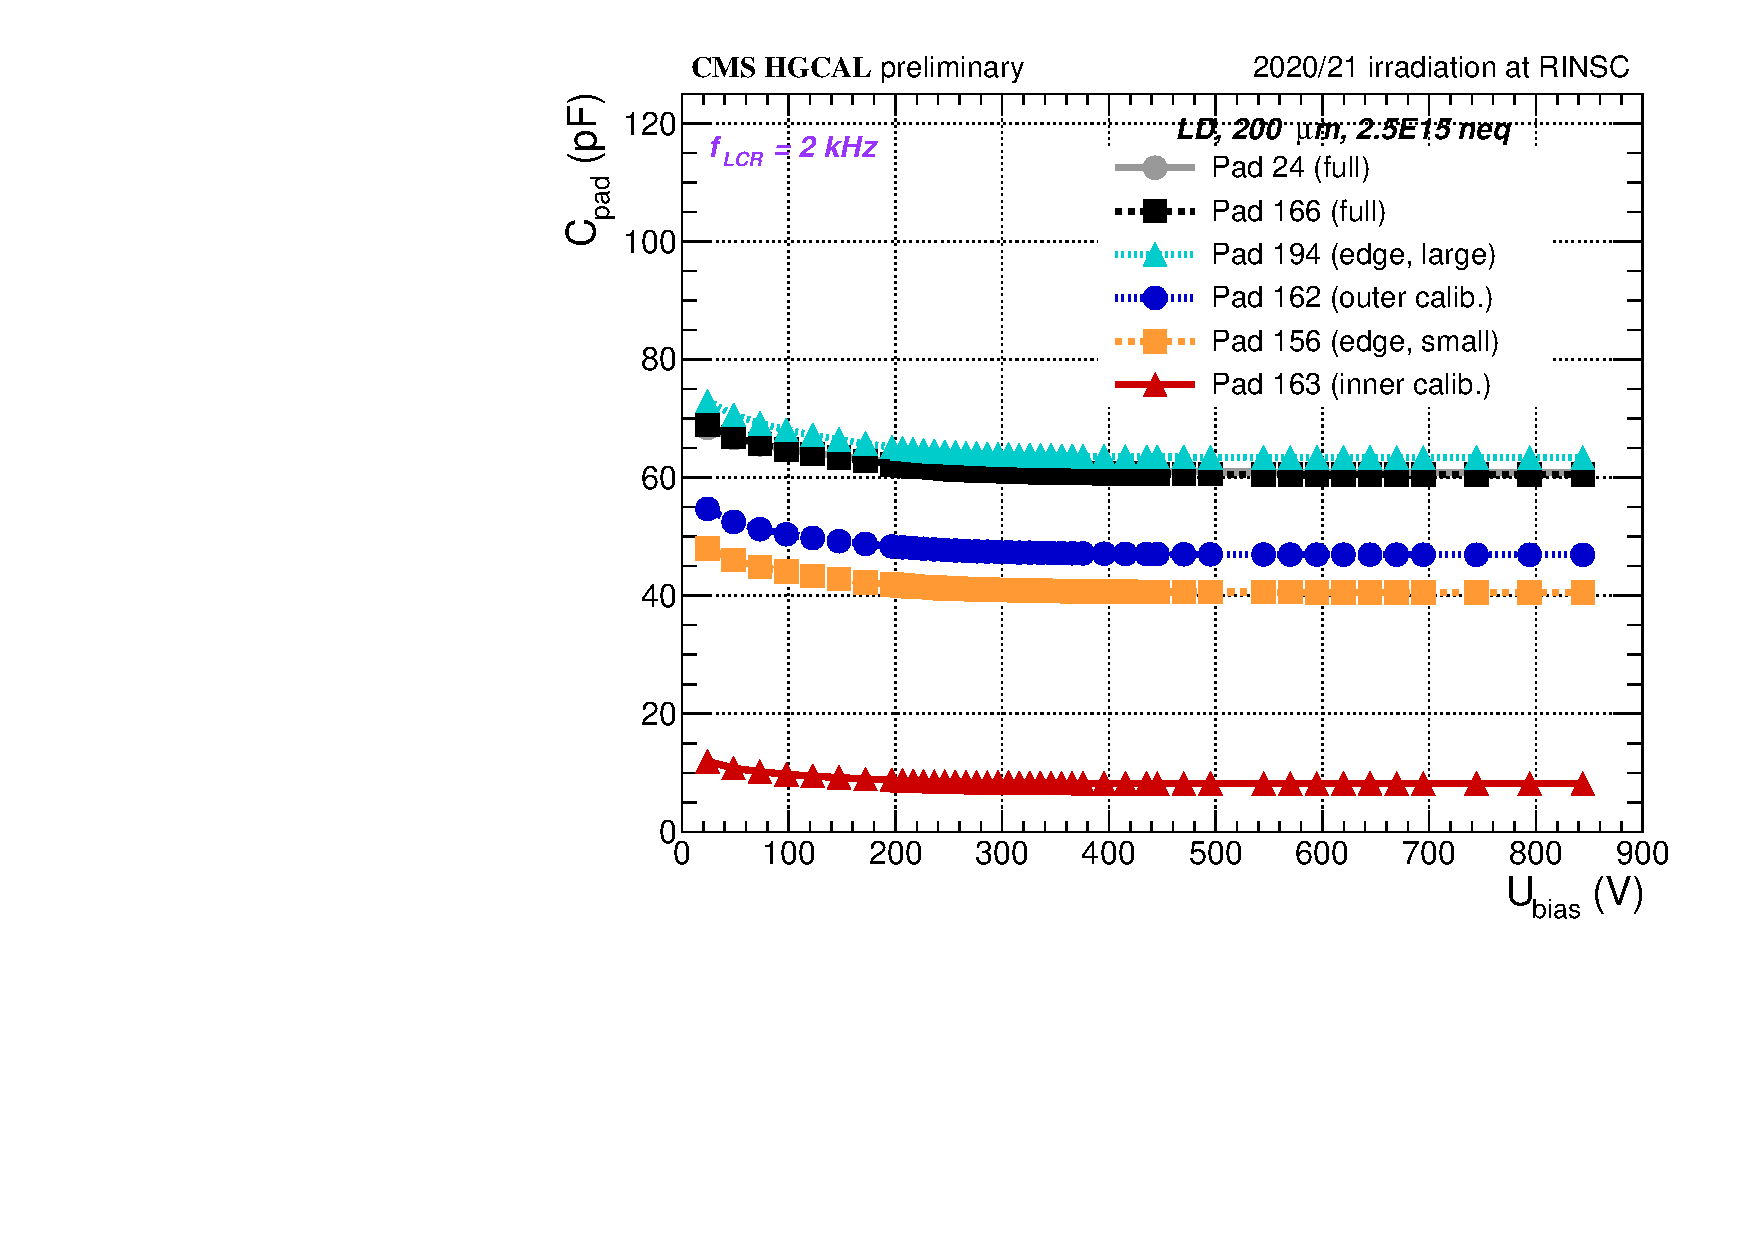
\includegraphics[width=0.999\textwidth]{plots/channel_cv/channel_CV_sensors_channels.pdf}
		\subcaption{
		}
		\label{plot:pad_CV_channels}
	\end{subfigure}
	\caption{
		Area- and thickness-normalised capacitances as a function of the effective bias voltage (a) for one central pad on six good sensors from all irradiation rounds, and (b) area-normalised for different pads with different geometries on one example sensor.
		The LCR frequency in these measurements was \SI{2}{\kilo\hertz}.
	}
\end{figure}

\begin{figure}
	\captionsetup[subfigure]{aboveskip=-1pt,belowskip=-1pt}
	\centering
	\begin{subfigure}[b]{0.49\textwidth}
		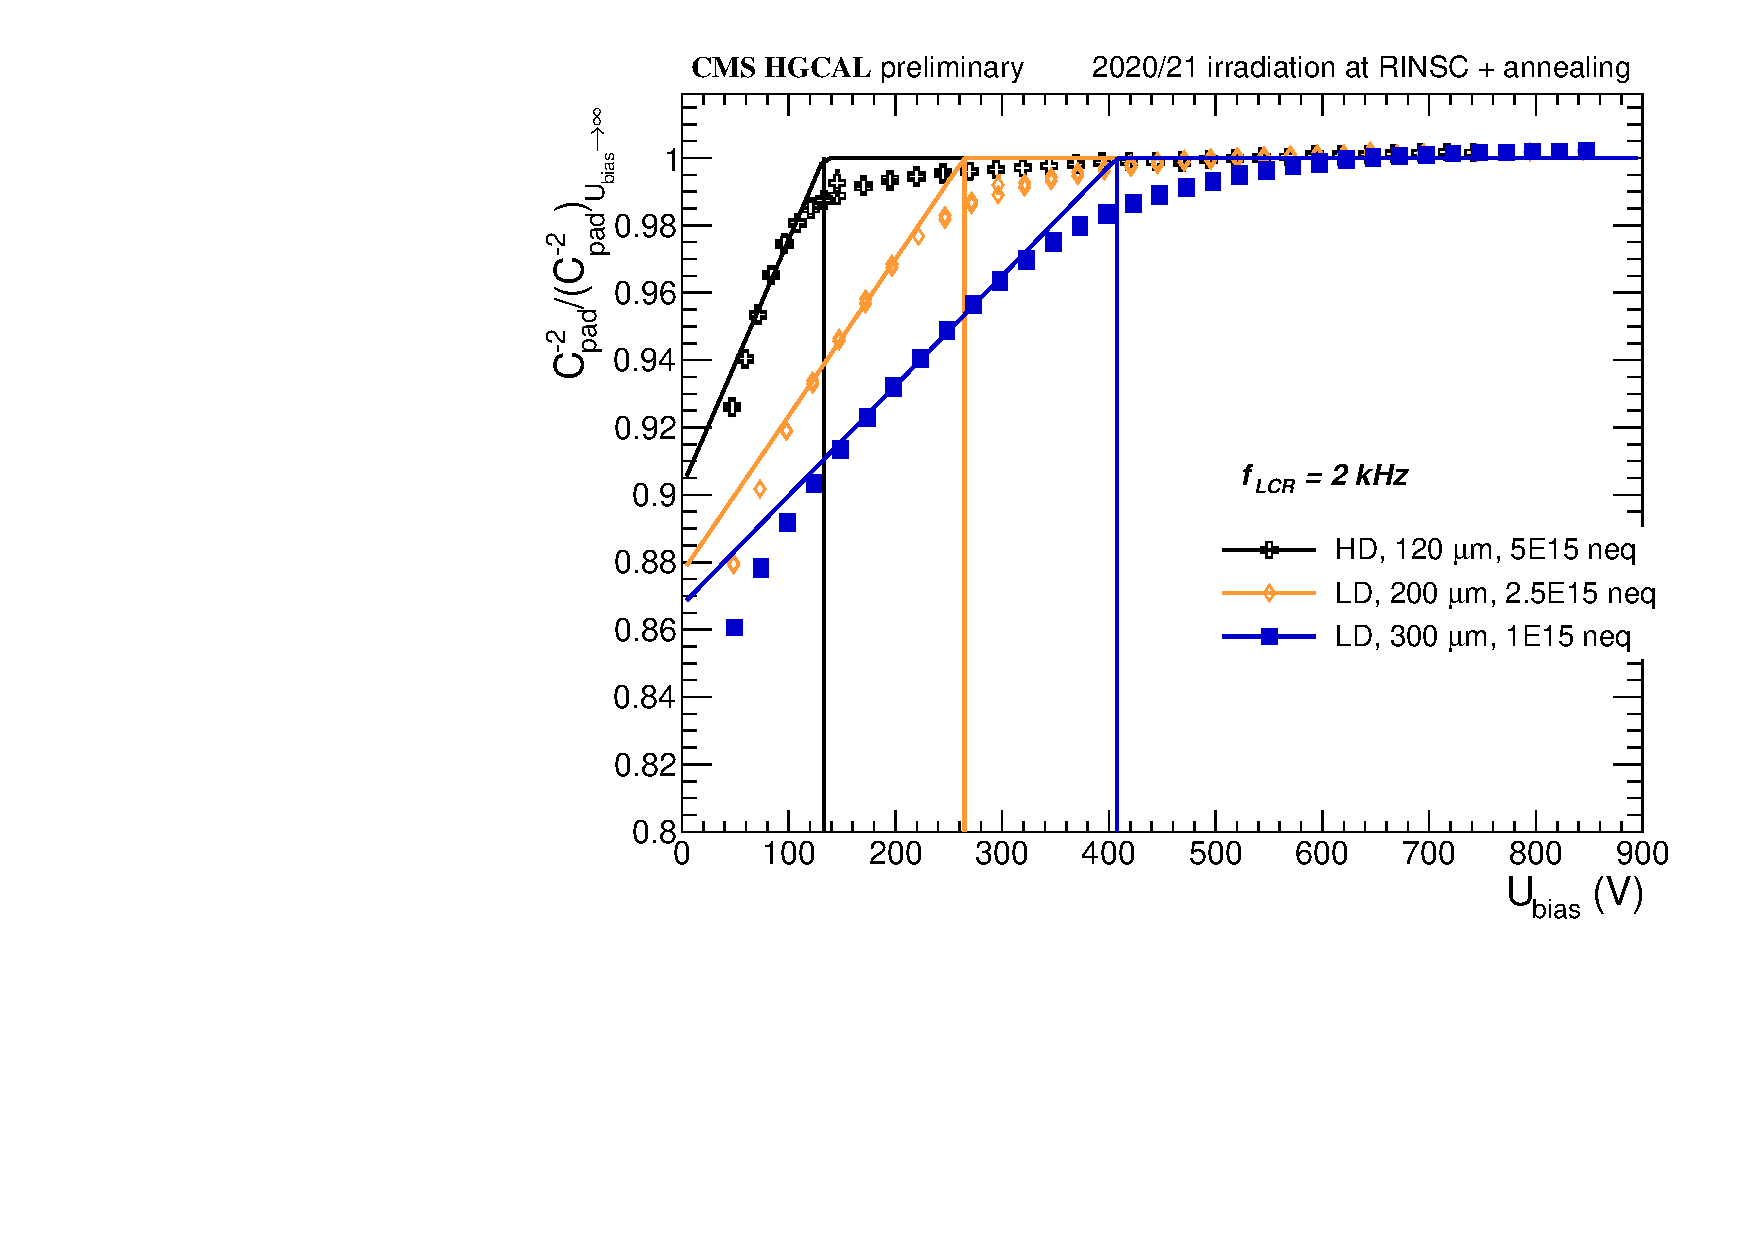
\includegraphics[width=0.999\textwidth]{plots/channel_cv/channel_invCV_sensors_sensors.pdf}
		\subcaption{
		}
		\label{plot:pad_invCV_sensor}
	\end{subfigure}
	\hfill
	\begin{subfigure}[b]{0.49\textwidth}
		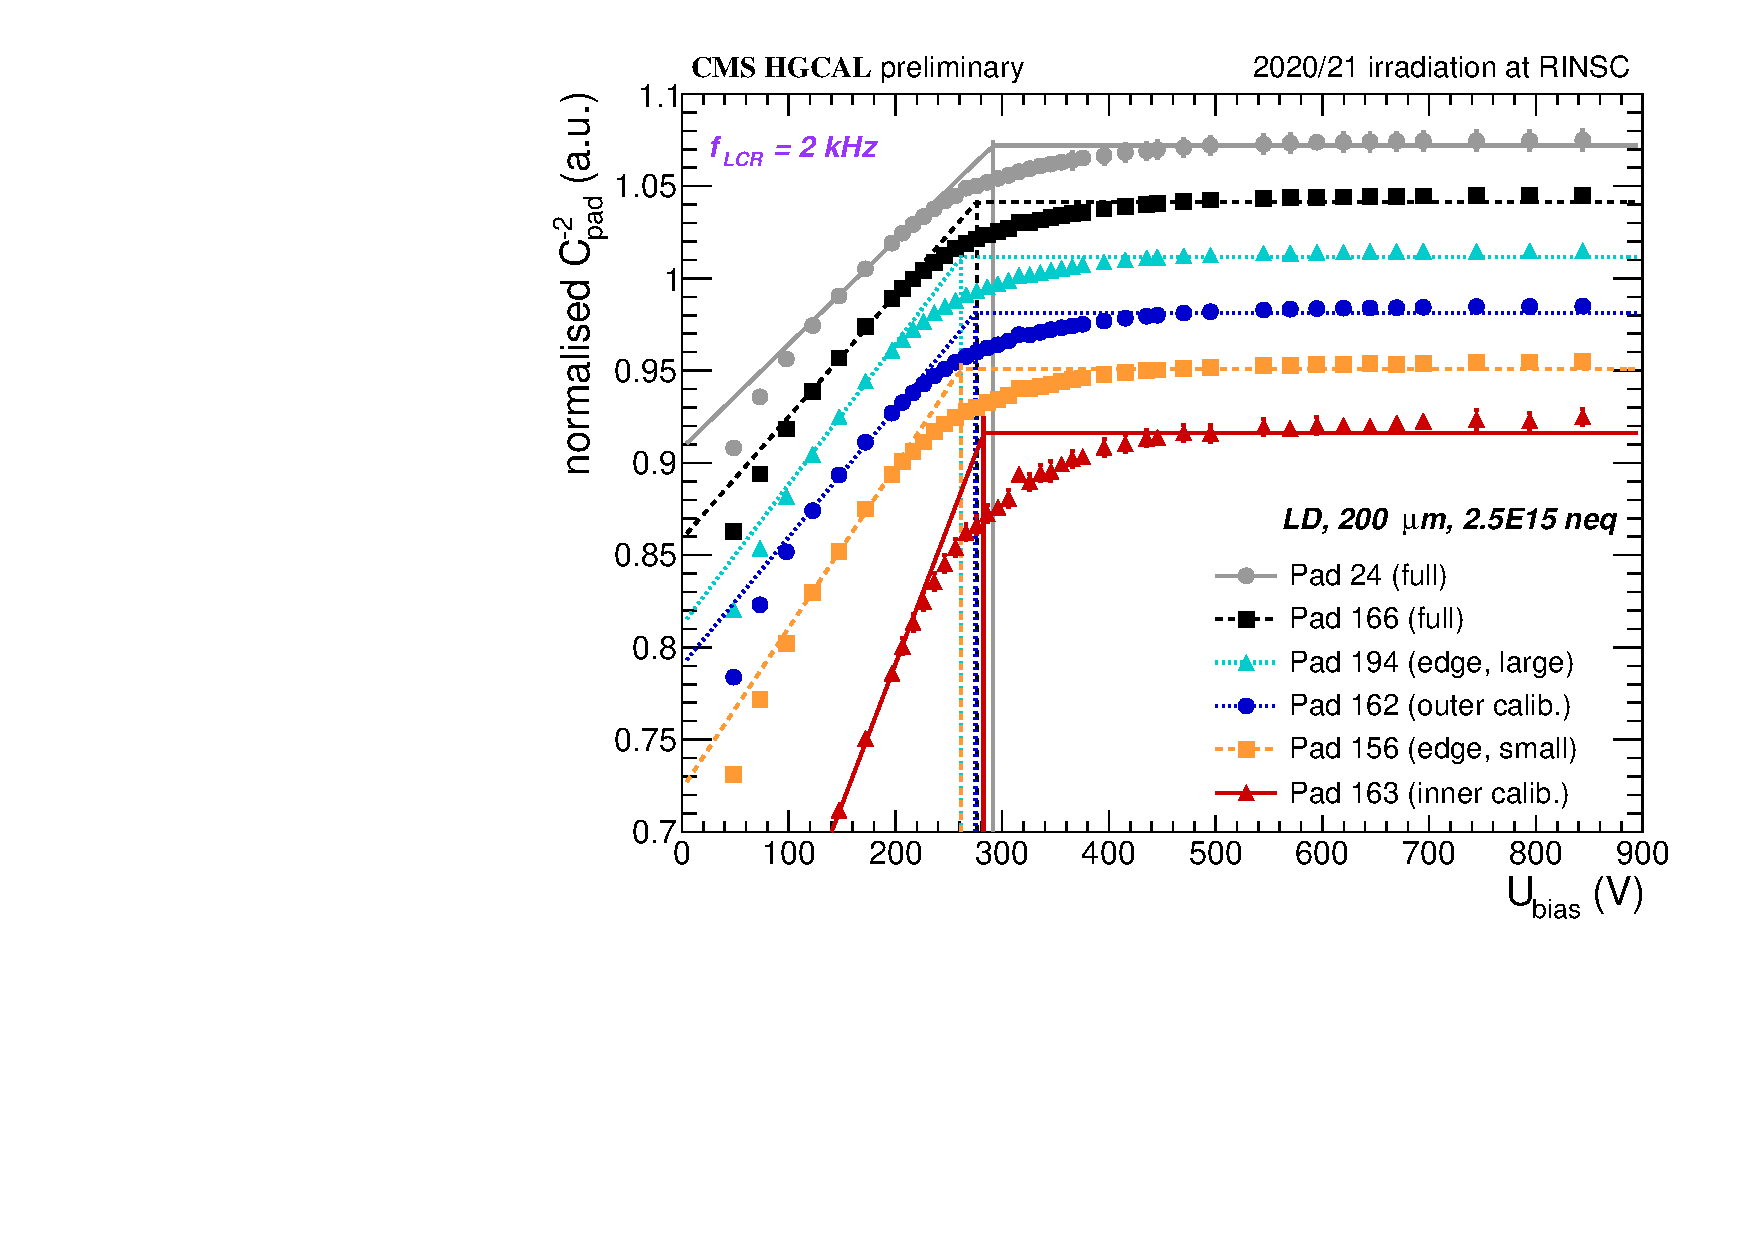
\includegraphics[width=0.999\textwidth]{plots/channel_cv/channel_invCV_sensors_channels.pdf}
		\subcaption{
		}
		\label{plot:pad_invCV_channels}
	\end{subfigure}
	\caption{
		Normalised squared-inverse capacitances as a function of the effective bias voltage for estimating the sensor depletion voltage (a) for one central pad on six good sensors from all irradiation rounds, and (b) for different pads with different geometries on one example sensor.
		The LCR frequency in these measurements was \SI{2}{\kilo\hertz}.
	}
\end{figure}


\begin{figure}
	\captionsetup[subfigure]{aboveskip=-1pt,belowskip=-1pt}
	\centering
	\begin{subfigure}[b]{0.49\textwidth}
		\centering
		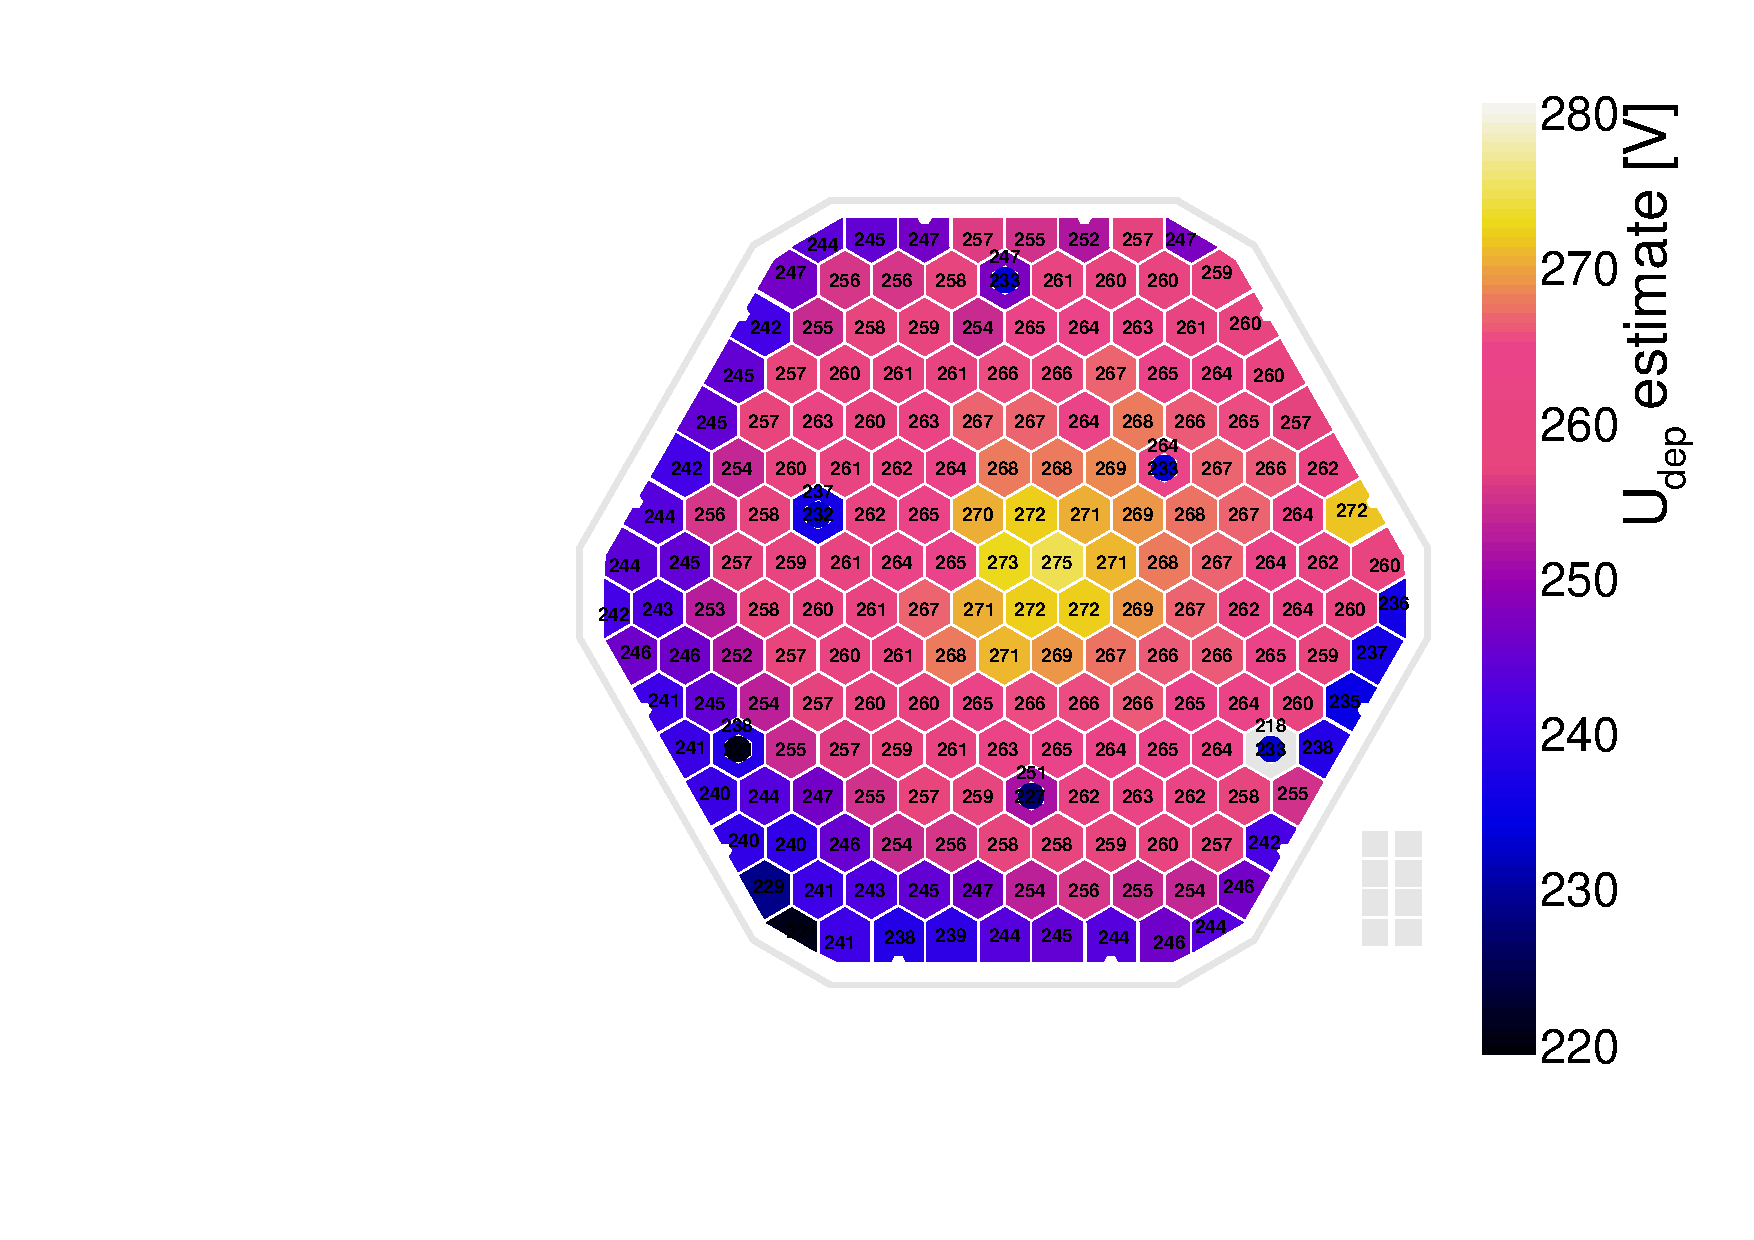
\includegraphics[width=0.7\textwidth]{plots/Vdep_hexplots/0541_04.pdf}
		\subcaption{
			}
			\label{plot:Vdep_hexplot_0541_04}
	\end{subfigure}
	\hfill
	\begin{subfigure}[b]{0.49\textwidth}
		\centering
		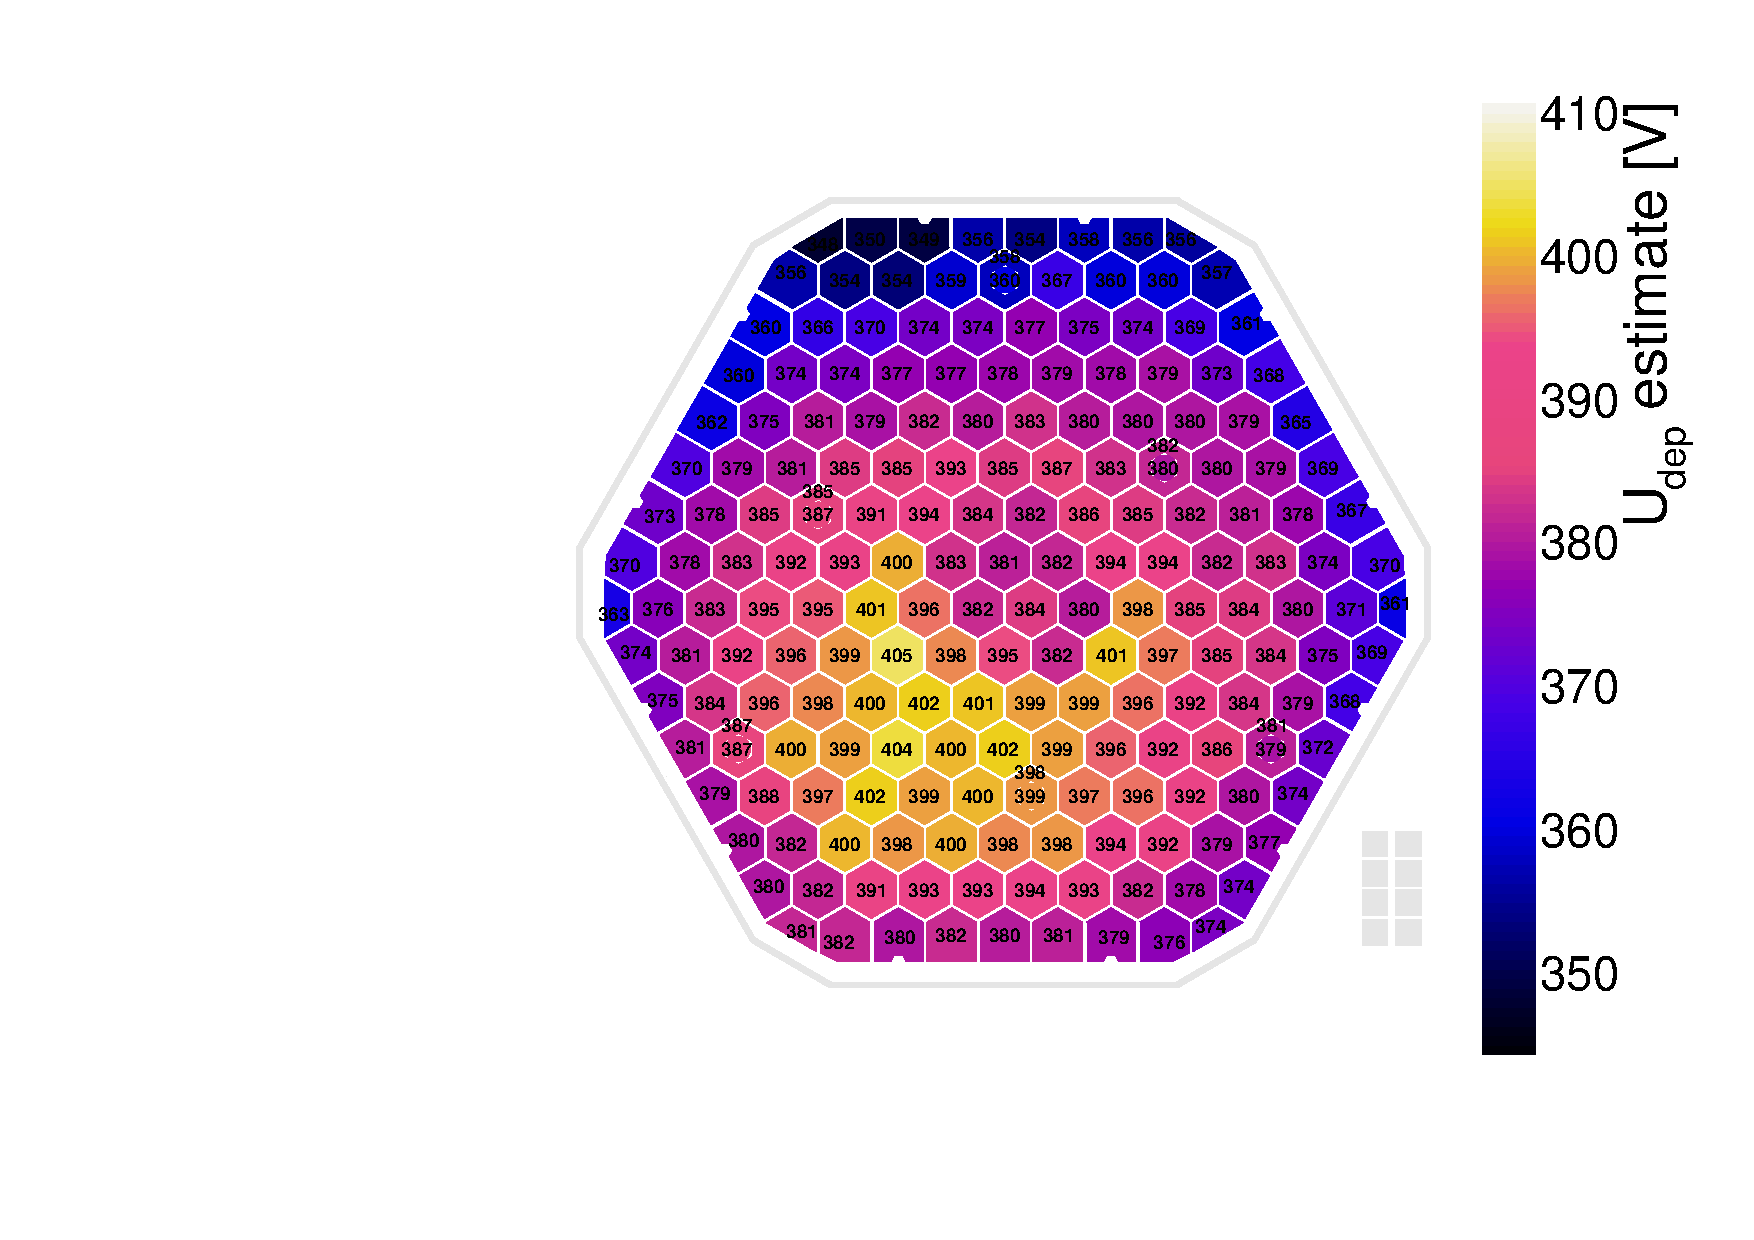
\includegraphics[width=0.7\textwidth]{plots/Vdep_hexplots/1002.pdf}
		\subcaption{
		}
		\label{plot:Vdep_hexplot_1002}
	\end{subfigure}	
	\caption{
		Per-pad depletion voltage estimates for (a) ..., (b). 
		Fluence profile visible, matches per-pad leakage current profiles cf.~\ref{plot:iv_hexplot_0541_04}, and~\ref{plot:iv_hexplot_1002}.
		Note the different colour scales.
	}
\end{figure}